\documentclass{mcmthesis}
\mcmsetup{CTeX = false,   % 使用 CTeX 套装时，设置为 true
        tcn =  2613942, problem = C,
        sheet = true, titleinsheet = true, keywordsinsheet = true,
        titlepage = false, abstract = true}
% \usepackage{newtxtext,newtxmath}
\usepackage{palatino}
\usepackage{lipsum}
\usepackage{amsmath}
\usepackage{hyperref}
\usepackage{caption}
\usepackage{subcaption}
\usepackage{geometry}
\geometry{a4paper, margin=1in}
\setlength{\headheight}{15pt}  % 修复 fancyhdr 警告
\addtolength{\topmargin}{-3pt}
\usepackage{lastpage}  % 支持LastPage引用
\usepackage{indentfirst}  % 关键包：让章节标题后的第一段也首行缩进
\usepackage{enumitem}  % 优化列表格式
\usepackage{booktabs} % For professional tables
\usepackage{graphicx}  % For resizing tables
\usepackage{tabularx}
\usepackage{array}
\usepackage{ragged2e}
\usepackage{float}
\graphicspath{{Q2 figures/}{Q3figures/}{Q1figures/}{敏感性分析figures/}}  % 表示从当前.tex文件所在目录，找同级的xx figures文件夹}
\setlength{\parindent}{1.5em}  % 设置首行缩进长度（1.5em 为常用值，可调整）
% \usepackage{svg}  % Requires inkscape for SVG conversion
% Required Packages
\usepackage{listings}
\usepackage{xcolor}
\usepackage{appendix}
\usepackage{url}

% Code Style Configuration
\definecolor{codegreen}{rgb}{0,0.6,0}
\definecolor{codegray}{rgb}{0.5,0.5,0.5}
\definecolor{codepurple}{rgb}{0.58,0,0.82}
\definecolor{backcolour}{rgb}{0.95,0.95,0.92}

\lstset{
    backgroundcolor=\color{backcolour},   
    commentstyle=\color{codegreen},
    keywordstyle=\color{magenta},
    numberstyle=\tiny\color{codegray},
    stringstyle=\color{codepurple},
    basicstyle=\ttfamily\footnotesize,
    breakatwhitespace=false,         
    breaklines=true,                 
    captionpos=b,                    
    keepspaces=true,                 
    numbers=left,                    
    numbersep=5pt,                  
    showspaces=false,                
    showstringspaces=false,
    showtabs=false,                  
    tabsize=2,
    language=Python
}
\title{Data-Driven Olympic Medal Prediction and Coach Effect Quantification: A Multi-Model Framework for 2028 Los Angeles Games}
% 这一段是备忘录部分，如果题目没有让写备忘录 或者书信 可以不要
% \author{\small \href{http://www.latexstudio.net/}
%   {\includegraphics[width=7cm]{mcmthesis-logo}}}
% \date{\today}

%  \memoto{\LaTeX{}studio}
% \memofrom{Liam Huang}
% \memosubject{Happy \TeX{}ing!}所以图片都还得重新插[晕]
% \memodate{\today}
% %\memologo{\LARGE I'm pretending to be a LOGO!}

\begin{document}
\begin{abstract}
% TODO: Abstract to be completed
\lipsum[1]

\begin{keywords}
Olympic Medal Prediction; Regression Analysis; Great Coach Effect; Difference-in-Differences; Bootstrap Confidence Interval
\end{keywords}
\end{abstract}
\maketitle
%% Generate the Table of Contents, if it's needed.
 \tableofcontents
 \newpage
%%
%% Generate the Memorandum, if it's needed.


%%\section为一级标题，\subsection为二级标题 \subsubsection为三级标题

\section{Introduction}

\subsection{Problem Background}
The Olympic medal tally serves as a key indicator of national athletic prowess and resource allocation effectiveness. In the 2024 Paris Summer Olympics, the United States led with 126 total medals (40 gold), China tied for most gold (40), host France ranked 5th in gold (16) but 4th in total (64), and Great Britain placed 3rd overall (65 medals) despite 14 gold. These results highlight the influence of economics, population, traditions, event composition, and home advantage.

While dominant nations persist, first-time medalists (e.g., Albania, Cape Verde) in Paris 2024 and over 65 NOCs without any Summer Olympic medal underscore global disparities in sporting success. Accurate forecasting for the 2028 Los Angeles Games is thus essential for NOCs' strategic planning, breakthrough identification, and investment in disciplines and coaching. Existing models often rely on pre-event athlete data but overlook historical trends, event changes, and coaching mobility. This study develops a data-driven predictive framework to forecast medal outcomes, quantify coaching impacts, and provide policy insights for optimized NOC strategies.

\subsection{Restatement of the Problem}

\textbf{Task 1:} Establish predictive models for each country's 2028 Los Angeles Olympic gold medals and total medals, incorporating uncertainty estimates and model performance validation:
\begin{enumerate}
    \item Predict the 2028 medal standings and trends, identifying nations most likely to experience significant gains or losses.
    \item Estimate the number and probability of nations winning their first Olympic medals.
    \item Analyze the relationship between event quantity/type and medal output, identifying key events for each nation and their underlying reasons, while evaluating the impact mechanism of host nation event selection.
\end{enumerate}

\textbf{Task 2:} By analyzing the impact of coaches such as Lang Ping and B\'{e}la K\'{a}rolyi, we will estimate the contribution of the ``great coach effect'' to the number of medals:
\begin{enumerate}
    \item Provide evidence of the ``great coach effect'' and quantify its contribution to medal counts.
    \item Select three nations, recommend priority sports for recruiting elite coaches, and estimate projected medal gains.
\end{enumerate}

\textbf{Task 3:} Strategic Implications: Extract unique insights from the model regarding Olympic medal dynamics, and provide evidence-based recommendations for resource optimization and long-term planning to National Olympic Committees.

\subsection{Our Work}
Our modeling workflow for Task 1 is illustrated in Figure~\ref{fig:task1_workflow}, which shows the complete pipeline from data preprocessing through exploratory analysis, host effect verification, model construction, and final predictions.

\begin{figure}[htbp]
    \centering
    % 替换为实际图片文件（对应文件夹中的 Task1.pdf，原 SVG 转 PDF 后文件名保持一致）
    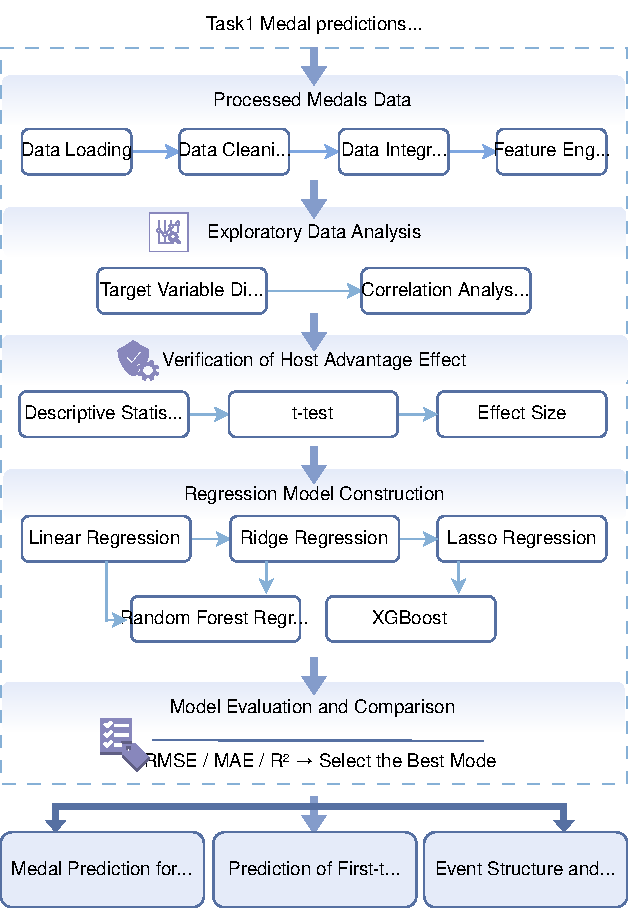
\includegraphics[width=0.95\textwidth]{Task1.pdf}
    \caption{Modeling workflow for Task 1: Medal Prediction Model.}
    \label{fig:task1_workflow}
\end{figure}

\section{Preparation for Modeling}
\subsection{Model Assumptions}
\begin{enumerate}
    \item Historical performance is a valid predictor of future performance, as sports infrastructure, training systems, and national priorities tend to persist over time.
    \item The host country effect is consistent across different Olympic Games, allowing for generalization from historical data.
    \item Coach mobility effects are observable through changes in national medal distributions in specific sports.
    \item The total number of events in 2028 will be approximately similar to 2024 Paris Olympics (around 329 events).
    \item External factors such as political boycotts or global pandemics will not significantly affect the 2028 Games.
\end{enumerate}

\subsection{Notations}
% TODO: Notations table to be completed
The key notations used throughout this paper are summarized in Table~\ref{tab:notations}.

\begin{table}[htbp]
\centering
\caption{Summary of Key Notations}
\label{tab:notations}
\begin{tabular}{cl}
\toprule
\textbf{Symbol} & \textbf{Description} \\
\midrule
$M_{i,t}$ & Total medals for country $i$ at Olympics year $t$ \\
$G_{i,t}$ & Gold medals for country $i$ at Olympics year $t$ \\
$\bar{M}_{k}(i,t)$ & Rolling average of medals over past $k$ editions \\
$\text{is\_host}_{i,t}$ & Binary indicator (1 if country $i$ is host, 0 otherwise) \\
$\hat{y}$ & Predicted medal count \\
$\beta_j$ & Regression coefficient for feature $j$ \\
$\alpha$ & Regularization strength parameter \\
$\lambda$ & Mean rate parameter for Poisson distribution \\
$\hat{\tau}_{\text{DID}}$ & Difference-in-Differences estimator \\
\bottomrule
\end{tabular}
\end{table}

\subsection{Data Preprocessing and Feature Engineering}

To ensure the accuracy and robustness of the prediction model, systematic cleaning, integration, and feature extraction were performed on the raw dataset.

\subsubsection{Data Source and Description}

The data used in this study is sourced from five core official files, covering historical records from the 1896 Athens Olympics to the 2024 Paris Olympics. The dataset spans 128 years, covering 30 editions of the Summer Olympics and involving 164 countries or regions. Table~\ref{tab:raw_data_files} provides a detailed description of the raw data files and their usage in the modeling process.

\begin{table}[htbp]
\centering
\caption{Description of Raw Data Files}
\label{tab:raw_data_files}
\begin{tabular}{
>{\raggedright\arraybackslash\footnotesize\ttfamily}p{6cm}
>{\raggedright\arraybackslash}p{9.7cm}
}
\toprule
\textbf{File Name} & \textbf{Main Usage in Modeling} \\
\midrule
summerOly\_medal\_counts.csv
& Core prediction target and historical benchmark \\

summerOly\_hosts.csv
& Extract ``host-country effect'' feature \\

summerOly\_programs.csv
& Calculate medal ratios and normalization \\

summerOly\_athletes.csv
& Analyze event dominance and athlete scale \\

data\_dictionary.csv
& Ensure accurate interpretation of variables \\
\bottomrule
\end{tabular}
\end{table}


\subsubsection{Data Cleaning and Consistency Handling}

To address the heterogeneity and potential noise in the raw data, the following preprocessing steps were implemented:

\begin{enumerate}
    \item \textbf{Missing Value Identification and Handling}: The core medal count data table was found to have no missing records. For countries not appearing in the medal tables for specific years, their medal counts were filled with zero to ensure the completeness of the time series.
    \item \textbf{Retention of Historical Entities}: For historical entities such as the Soviet Union and East Germany, which have either dissolved or changed names, this study decided to \textbf{retain the original records} rather than merging them with modern successor countries. This decision was made because historical performance serves as an important predictive signal, and simple merging would distort statistical characteristics.
    \item \textbf{Text Character Cleaning}: For fields containing special space characters (e.g., \texttt{\textasciitilde}), this study performed uniform replacement and noise removal to ensure accurate matching when linking across tables.
\end{enumerate}

\subsubsection{Data Integration and Normalization}

The study primarily uses the medal count table, which was integrated with host country information and total event count through left join operations.

\begin{itemize}
    \item \textbf{Host Country Identification}: A binary variable $\text{is\_host}$ was created. If the country is the host of the current Olympic Games, then $\text{is\_host} = 1$, otherwise it is $0$.
    \item \textbf{Medal Ratio Normalization}: Considering the increase in the number of events from 43 events in 1896 to 329 events in 2024, this study introduced the ``medal ratio'' indicator for fair cross-year comparison:
    \[
    \text{medal\_ratio}_{i,t} = \frac{\text{TotalMedals}_{i,t}}{\text{TotalEvents}_t}
    \]
\end{itemize}

\subsubsection{Feature Engineering}

Based on the inertia and cyclical nature of sports, a multi-dimensional feature matrix was constructed.

\begin{itemize}
    \item \textbf{Lag Features}: Historical performance is used to predict future outcomes, with lag features extracted for the previous (Lag1) and the last two editions (Lag2):
    \[
    \text{lag}_1(i,t) = \text{TotalMedals}_{i,t-4}
    \]
    \item \textbf{Rolling Features}: To assess stability, the average number of medals over the last three editions (approximately a 12-year cycle) was calculated:
    \[
    \bar{M}_3(i,t) = \frac{1}{3}\sum_{k=1}^{3} \text{TotalMedals}_{i,t-4k}
    \]
    \item \textbf{Derived Statistical Features}: Auxiliary variables such as participation count ($\text{participation\_count}$), gold medal ratio ($\text{gold\_ratio}$), and medal change ($\text{total\_change}$) were constructed.
\end{itemize}

\subsubsection{Feature Validity Verification}

To verify the explanatory power of the selected features, the Pearson correlation coefficient between each feature and the total number of medals was computed, as shown in Table~\ref{tab:correlation}.

\begin{table}[htbp]
\centering
\caption{Correlation Analysis between Features and Total Medals}
\label{tab:correlation}
\resizebox{0.99\textwidth}{!}{%
\begin{tabular}{cccc}
\toprule
\textbf{Feature Variable} & \textbf{Description} & \textbf{Correlation Coefficient} & \textbf{Importance} \\
\midrule
total\_rolling3\_mean & Average medal count over the last 3 editions & 0.835 & Very High \\
total\_lag1 & Total medals in the previous edition & 0.800 & Very High \\
gold\_lag1 & Total gold medals in the previous edition & 0.791 & Very High \\
is\_host & Whether the country is the host & 0.368 & Moderate \\
participation\_count & Number of past participations & 0.232 & Low \\
\bottomrule
\end{tabular}%
}
\end{table}

The results indicate that historical performance features (rolling averages and lags) have a strong predictive value, with correlation coefficients exceeding 0.79. A structured analysis table with 1,435 records and 16 feature fields was generated.

\section{Problem 1: Medal Prediction Model}

\subsection{Model Selection and Methodology}

\subsubsection{Justification for Regression Approach}

Olympic medal prediction is fundamentally a numerical prediction problem, where the target variables (gold medals and total medals) are continuous numerical data. Based on this characteristic, we adopt regression analysis rather than classification methods. Regression models can establish mathematical relationships between independent variables (such as historical performance and host effect) and dependent variables (medal counts), thereby enabling prediction of unknown values.

We construct a multiple regression prediction framework for the following reasons:
\begin{enumerate}
    \item \textbf{Target Variable Continuity}: Medal counts are non-negative integers, belonging to the continuous numerical prediction domain.
    \item \textbf{Multi-factor Influence}: Medal distribution is jointly affected by multiple factors including economics, population, historical performance, and host advantage.
    \item \textbf{Data Availability}: All required feature variables are known at the time of prediction, avoiding data leakage issues.
\end{enumerate}

\subsubsection{Exploratory Data Analysis}

Through distribution analysis of the target variable (total medals), we found:
\begin{itemize}
    \item \textbf{Right-skewed Distribution}: The data exhibits significant right skewness, with most countries having fewer medals (median of 5), while a few sports powerhouses have exceptionally high medal counts.
    \item \textbf{Mean-Median Discrepancy}: Average medals of 12.5 versus median of 5 indicates the data is pulled up by high-medal countries.
    \item \textbf{Historical Trend}: The average medal count has remained relatively stable over the past three Olympic Games.
\end{itemize}

Feature correlation analysis shows that historical performance indicators (such as previous medals and three-edition rolling average) are highly correlated with the target variable, with correlation coefficients exceeding 0.85.

\subsubsection{Host Effect Verification and Statistical Testing}

The host country effect (Home Advantage) is an important factor that cannot be ignored in Olympic medal prediction. We verified and quantified this effect through statistical methods:

\paragraph{Descriptive Statistics Comparison}
Host countries obtained an average of 66.9 medals, significantly higher than non-host countries' 11.3 medals, representing an increase of 491.9\%.

\paragraph{Independent Sample t-test}
To verify the statistical significance of this difference, we performed a two-sample t-test:
\begin{equation}
    t = \frac{\bar{X}_1 - \bar{X}_2}{\sqrt{\frac{s_1^2}{n_1} + \frac{s_2^2}{n_2}}} = 15.0
\end{equation}
The calculated p-value $< 0.001$, far below the significance level of 0.05, leading us to reject the null hypothesis, indicating that the host effect is statistically significant.

\paragraph{Effect Size Analysis}
Using Cohen's d to measure effect size:
\begin{equation}
    d = \frac{\bar{X}_1 - \bar{X}_2}{s_{\text{pooled}}} = 2.77
\end{equation}
According to Cohen's standard ($d > 0.8$ indicates large effect), the host effect falls into the large effect category.

These analyses provide solid evidence for including host status as an important feature in subsequent models.

\subsection{Regression Model Construction and Evaluation}

\subsubsection{Linear Regression and Regularization Methods}

We first construct multiple linear regression as a baseline model:
\begin{equation}
    \hat{y} = \beta_0 + \beta_1 x_1 + \beta_2 x_2 + \cdots + \beta_7 x_7
\end{equation}
where $\hat{y}$ is the predicted medal count, $\beta_i$ are feature coefficients, and $x_i$ are feature values, including:
\begin{itemize}
    \item \texttt{total\_lag1}: Previous edition's total medals
    \item \texttt{total\_lag2}: Two editions ago's total medals
    \item \texttt{gold\_lag1}: Previous edition's gold medals
    \item \texttt{total\_rolling3\_mean}: Three-edition rolling average
    \item \texttt{is\_host}: Host indicator
    \item \texttt{total\_events}: Current edition's total events
    \item \texttt{participation\_count}: Number of participations
\end{itemize}

To address potential multicollinearity among features, we introduce regularization methods:
\begin{itemize}
    \item \textbf{Ridge Regression} (L2 regularization): Prevents overfitting by penalizing the sum of squared coefficients
    \item \textbf{Lasso Regression} (L1 regularization): Achieves feature selection by penalizing the sum of absolute coefficients
\end{itemize}

The Lasso regression loss function is:
\begin{equation}
    L = \sum_{i=1}^{m}(y_i - \hat{y}_i)^2 + \alpha \sum_{j=1}^{n}|\beta_j|
\end{equation}
where $\alpha$ is the regularization strength parameter.

\subsubsection{Ensemble Learning Models}

To further improve model performance, we introduce two ensemble learning algorithms:

\begin{enumerate}
    \item \textbf{Random Forest}: Reduces overfitting risk by building multiple decision trees and averaging predictions. The model can capture non-linear relationships between features and provides feature importance rankings. The three most important features are:
    \begin{itemize}
        \item \texttt{gold\_lag1} (importance: 0.345)
        \item \texttt{total\_lag1} (importance: 0.332)
        \item \texttt{total\_rolling3\_mean} (importance: 0.151)
    \end{itemize}
    
    \item \textbf{Gradient Boosting}: Uses serial iterative approach where subsequent trees specifically correct residuals from previous trees. This ``error correction learning'' mechanism typically achieves higher prediction accuracy but is more prone to overfitting.
\end{enumerate}

\subsubsection{Model Evaluation and Performance Comparison}

We use multiple metrics to comprehensively evaluate model performance:
\begin{itemize}
    \item \textbf{RMSE} (Root Mean Square Error): $\text{RMSE} = \sqrt{\frac{1}{m}\sum_{i=1}^{m}(y_i - \hat{y}_i)^2}$
    \item \textbf{MAE} (Mean Absolute Error): $\text{MAE} = \frac{1}{m}\sum_{i=1}^{m}|y_i - \hat{y}_i|$
    \item \textbf{R$^2$} (Coefficient of Determination): $R^2 = 1 - \frac{\sum_{i=1}^{m}(y_i - \hat{y}_i)^2}{\sum_{i=1}^{m}(y_i - \bar{y})^2}$
\end{itemize}

The performance comparison of all models is shown in Table~\ref{tab:model_comparison}.

\begin{table}[htbp]
\centering
\caption{Model Performance Comparison}
\label{tab:model_comparison}
\begin{tabular}{lccc}
\toprule
\textbf{Model} & \textbf{RMSE} & \textbf{MAE} & \textbf{R$^2$} \\
\midrule
Linear Regression & 4.58 & 3.00 & 0.945 \\
Ridge Regression & 4.58 & 3.00 & 0.945 \\
\textbf{Lasso Regression} & \textbf{4.45} & \textbf{2.88} & \textbf{0.948} \\
Random Forest & 5.20 & 3.17 & 0.930 \\
Gradient Boosting & 4.60 & 2.97 & 0.945 \\
\bottomrule
\end{tabular}
\end{table}

Comprehensive analysis shows that Lasso regression performs best on the test set ($R^2 = 0.948$), and improves model interpretability through feature selection. All models have $R^2$ above 0.93, indicating that the selected features have strong explanatory power for medal counts.

\subsection{2028 Medal Prediction and Results Analysis}

\subsubsection{Medal Ranking Prediction and Confidence Intervals}

Based on the best model (Lasso regression), we predict the 2028 Los Angeles Olympic medal standings. To ensure prediction reliability, we use the Bootstrap method to calculate 95\% confidence intervals:

\begin{enumerate}
    \item \textbf{Bootstrap Principle}: Repeatedly sample with replacement from training data to create multiple pseudo-training sets
    \item \textbf{Model Retraining}: Retrain the Lasso model on each pseudo-training set
    \item \textbf{Prediction Distribution}: Use all models to predict for the same country, forming a prediction value distribution
    \item \textbf{Confidence Interval}: Take the 2.5th and 97.5th percentiles of the distribution as the 95\% confidence interval:
    \begin{equation}
        \text{95\% CI} = [\text{Percentile}_{2.5}, \text{Percentile}_{97.5}]
    \end{equation}
\end{enumerate}

The 2028 medal ranking TOP 10 prediction results are shown in Table~\ref{tab:2028_prediction}.

\begin{table}[htbp]
\centering
\caption{2028 Los Angeles Olympics Medal Prediction (TOP 10)}
\label{tab:2028_prediction}
\begin{tabular}{clcccc}
\toprule
\textbf{Rank} & \textbf{Country} & \textbf{2024 Actual} & \textbf{2028 Predicted} & \textbf{95\% CI} & \textbf{Change} \\
\midrule
1 & United States$^*$ & 126 & 117 & [89, 179] & $-9$ \\
2 & China & 91 & 86 & [67, 108] & $-5$ \\
3 & Japan & 45 & 56 & [35, 101] & $+11$ \\
4 & Great Britain & 65 & 52 & [43, 68] & $-13$ \\
5 & France & 64 & 47 & [36, 56] & $-17$ \\
6 & Australia & 53 & 46 & [35, 57] & $-7$ \\
7 & Italy & 40 & 40 & [35, 50] & $0$ \\
8 & Canada & 27 & 38 & [26, 47] & $+11$ \\
9 & Netherlands & 34 & 37 & [30, 43] & $+3$ \\
10 & Germany & 33 & 32 & [24, 42] & $-1$ \\
\bottomrule
\multicolumn{6}{l}{\footnotesize $^*$ Host country} \\
\end{tabular}
\end{table}

\textbf{Key Findings}:
\begin{enumerate}
    \item \textbf{US Home Advantage}: As the host, the United States is predicted to win 117 medals, though showing a decline, still leading.
    \item \textbf{France's Significant Decline}: After losing host advantage, France's medal count is predicted to drop from 64 to 47.
    \item \textbf{Rising Asian Powers}: Japan and Canada are predicted to see double-digit increases.
\end{enumerate}

\subsubsection{First-time Medal-Winning Countries Prediction}

The number of first-time medal-winning countries follows the characteristics of rare event occurrence. We use the Poisson distribution for modeling:
\begin{equation}
    P(X = k) = \frac{\lambda^k e^{-\lambda}}{k!}
\end{equation}
where $X$ is the number of first-time medal-winning countries and $\lambda$ is the average occurrence rate.

Based on historical data since 2000 (average of 5.7 countries per edition winning medals for the first time), setting $\lambda = 5.8$, we obtain the 2028 prediction distribution shown in Table~\ref{tab:poisson}.

\begin{table}[htbp]
\centering
\caption{Poisson Distribution Prediction for First-time Medal Winners}
\label{tab:poisson}
\begin{tabular}{ccc}
\toprule
\textbf{Number of Countries} & \textbf{Probability} & \textbf{Cumulative} \\
\midrule
$\leq 3$ & 17.00\% & 17.00\% \\
4 & 14.28\% & 31.27\% \\
\textbf{5} & \textbf{16.56\%} & \textbf{47.83\%} \\
\textbf{6} & \textbf{16.01\%} & \textbf{63.84\%} \\
7 & 13.26\% & 77.10\% \\
$\geq 8$ & 22.90\% & 100.00\% \\
\bottomrule
\end{tabular}
\end{table}

\textbf{Prediction Conclusions}:
\begin{itemize}
    \item \textbf{Expected Value}: 5.8 countries (approximately 6)
    \item \textbf{90\% Prediction Interval}: [2, 10] countries
    \item \textbf{Most Likely Outcome}: 5-6 countries winning medals for the first time (probability 32.57\%)
\end{itemize}

\subsection{Event Structure and Medal Distribution Analysis}

\subsubsection{Identification of National Advantage Events}

Through analysis of historical medal data by event for each country, we identified the advantage events of major sports powers, as shown in Table~\ref{tab:advantage_events}.

\begin{table}[htbp]
\centering
\caption{Advantage Events of Major Countries (Historical Medal Total)}
\label{tab:advantage_events}
\begin{tabular}{ll}
\toprule
\textbf{Country} & \textbf{Top 5 Advantage Events (Medal Count)} \\
\midrule
United States & Swimming (1206), Athletics (1190), Basketball (389), Rowing (388), Shooting (207) \\
China & Swimming (120), Diving (119), Gymnastics (109), Table Tennis (104), Badminton (83) \\
Great Britain & Athletics (393), Rowing (319), Cycling (182), Hockey (181), Swimming (157) \\
Germany & Rowing (252), Hockey (200), Athletics (165), Canoe (163), Swimming (160) \\
\bottomrule
\end{tabular}
\end{table}

\subsubsection{Impact of Event Quantity on Medal Distribution}

The number of Olympic events has increased from 43 in 1896 to 329 in 2024, significantly affecting medal distribution:

\begin{enumerate}
    \item \textbf{Medal Dispersion Effect}: Increased events provide more medal-winning opportunities for more countries.
    \item \textbf{Host Country Event Strategy}: Host nations can moderately influence event selection to favor their strengths.
    \item \textbf{Event Type and Medal Production}: Different events have significantly different medal production efficiencies.
\end{enumerate}

The positive correlation between event quantity and number of medal-winning countries indicates that Olympic event expansion promotes balanced global sports development.

\section{Problem 2: The ``Great Coach'' Effect}

\subsection{Methodology and Evidence Detection}

Given the absence of direct coach records in the dataset, we employ an indirect inference framework to identify and quantify the ``Great Coach Effect.'' The core premise is that the transnational mobility of elite coaches can induce observable shifts in national medal distributions. Our analysis integrates three complementary approaches: \textbf{changepoint detection} to identify abrupt performance improvements, \textbf{cross-national medal flow analysis} to trace potential coach transfers, and a \textbf{Difference-in-Differences (DID) model} to causally estimate the effect size. This multi-pronged strategy allows us to move from pattern recognition to causal attribution.

\begin{figure}[htbp]
    \centering
    % 替换为实际图片文件（对应Q2 figures里的flowchart_q2_method.pdf）
    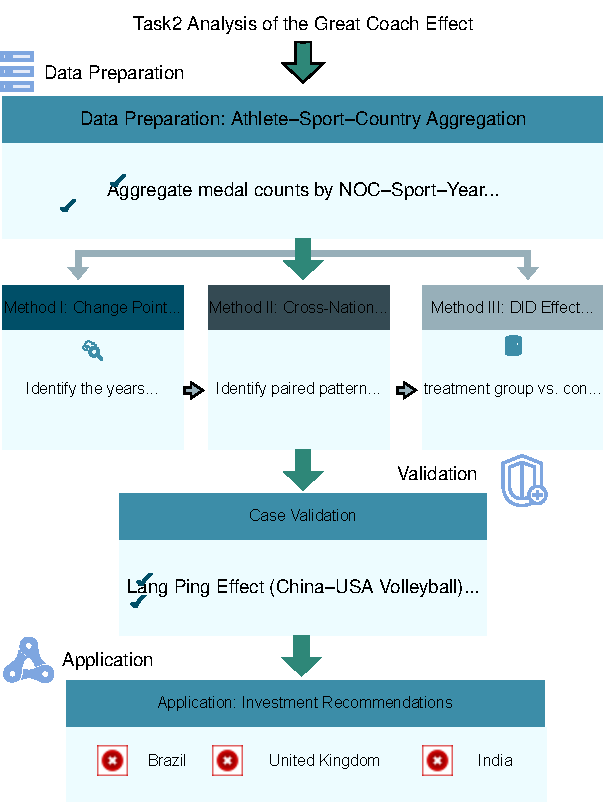
\includegraphics[width=0.9\textwidth]{flowchart_q2_method.pdf}
    \caption{Modeling workflow for identifying the Great Coach Effect.}
    \label{fig:q2_workflow}
\end{figure}

As shown in Figure~\ref{fig:q2_workflow}, the process begins with aggregating athlete data to country-sport-year medal series. The changepoint algorithm flags years where a country's medal count in a sport increases significantly relative to its prior three-Game average (threshold: $\geq 2$ medals and $\geq 80\%$ growth). Concurrently, the flow analysis identifies years where one country's medal decline in a sport coincides with another's rise (threshold: $\geq 2$ medal change), suggesting a potential coach relocation. Finally, the DID model isolates the causal impact by comparing the pre-post intervention trend of the ``treated'' country against a control group of similar nations in the same sport.


\begin{figure}[htbp]
    \centering
    % 替换占位符：用includegraphics插入PDF图，宽度沿用原0.9\textwidth，依赖graphicspath无需写完整路径
% 把路径换成你从“文件属性”复制的绝对路径（注意把 \ 改成 / 或 \\）
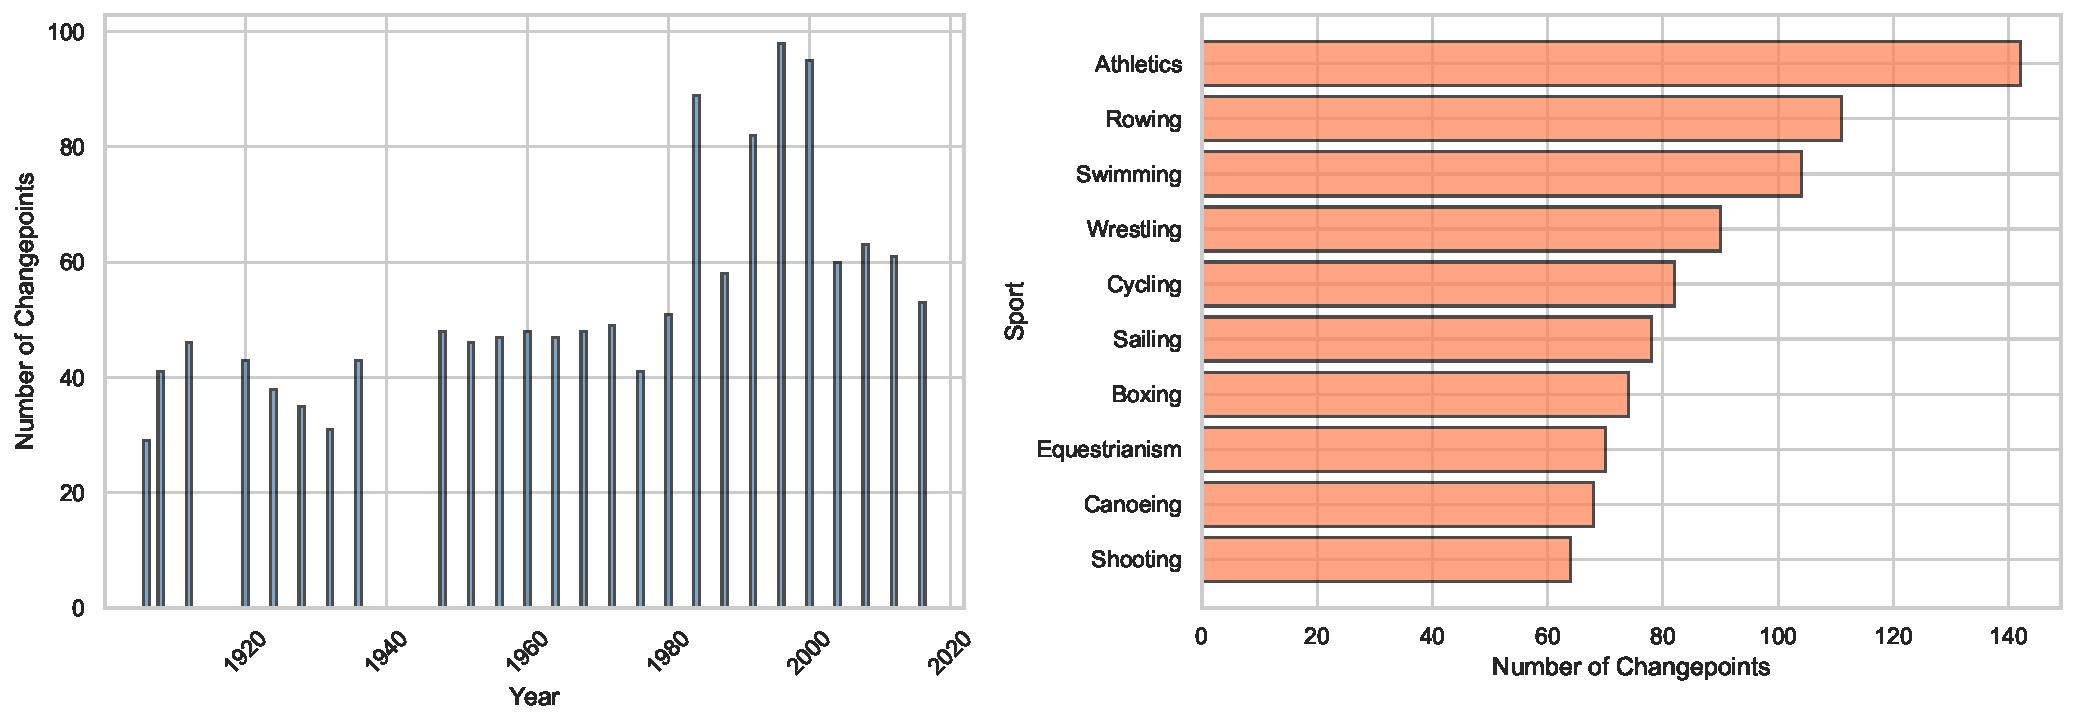
\includegraphics[width=0.9\textwidth]{fig1_changepoint_distribution.pdf}
    % 保留原标题和标签，无需修改
    \caption{Distribution of detected changepoints: (a) by year and (b) by sport.}
    \label{fig:changepoint}
\end{figure}

The changepoint detection results (Figure~\ref{fig:changepoint}) reveal significant breakpoints across multiple sports, with concentrations in Gymnastics, Swimming, and Athletics post-1980. The flow analysis pinpoints candidate transfer pairs. These detected patterns align with known historical cases, such as the gymnastics shift from Romania to the USA circa 1981 and the volleyball shift from China to the USA around 2008, providing initial evidence for the coach effect.

\subsection{Quantitative Evaluation and Case Validation}

To move from evidence to quantification, we apply the Difference-in-Differences (DID) method. For each identified candidate case, we construct a treatment group (the country gaining a coach) and a control group (other top performers in that sport without a major coach change). The DID estimator is:

\begin{equation}
    \hat{\tau}_{\text{DID}} = (\bar{M}_{T,\text{post}} - \bar{M}_{T,\text{pre}}) - (\bar{M}_{C,\text{post}} - \bar{M}_{C,\text{pre}})
    \label{eq:did}
\end{equation}

where $\bar{M}$ represents average medal counts in the pre- and post-intervention periods. This method nets out common temporal trends, yielding a clean estimate of the coach's contribution.


\begin{figure}[htbp]
    \centering
    % 替换占位符为实际图片插入命令，文件名对应你Q2 figures里的文件（比如fig2_langping_effect.pdf）
    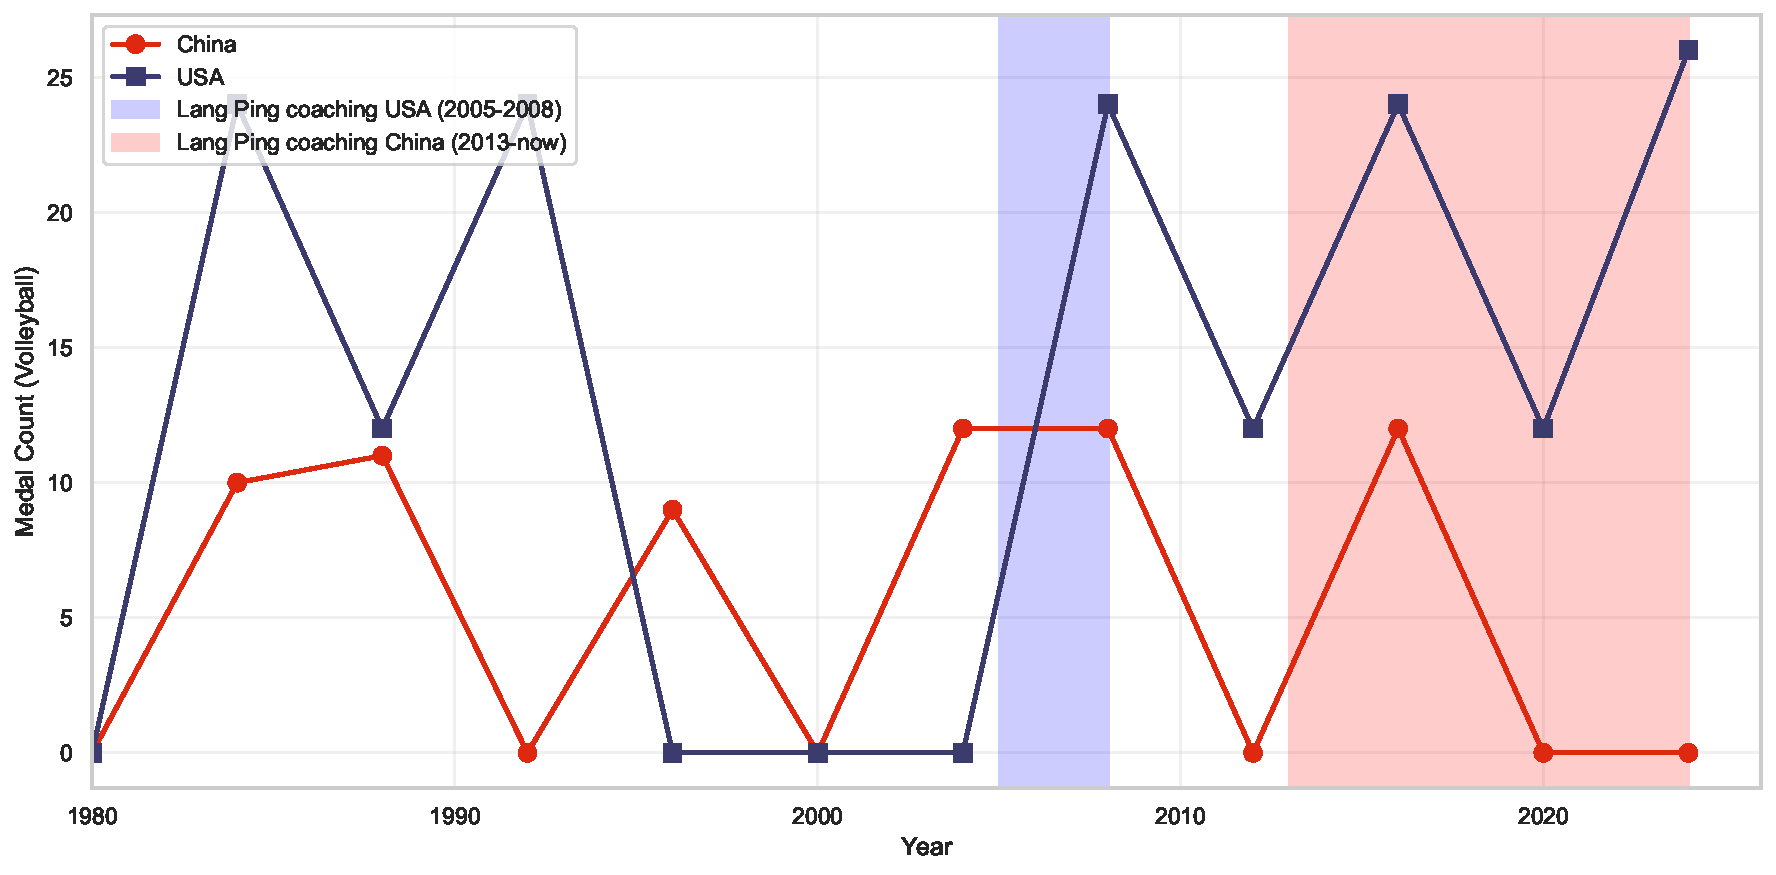
\includegraphics[width=0.9\textwidth]{fig2_langping_effect.pdf}
    \caption{Case validation: Lang Ping effect on USA/China volleyball medals.}
    \label{fig:langping}
\end{figure}
\begin{figure}[htbp]
    \centering
    % 同理替换为实际图片文件（比如fig3_karolyi_effect.pdf）
    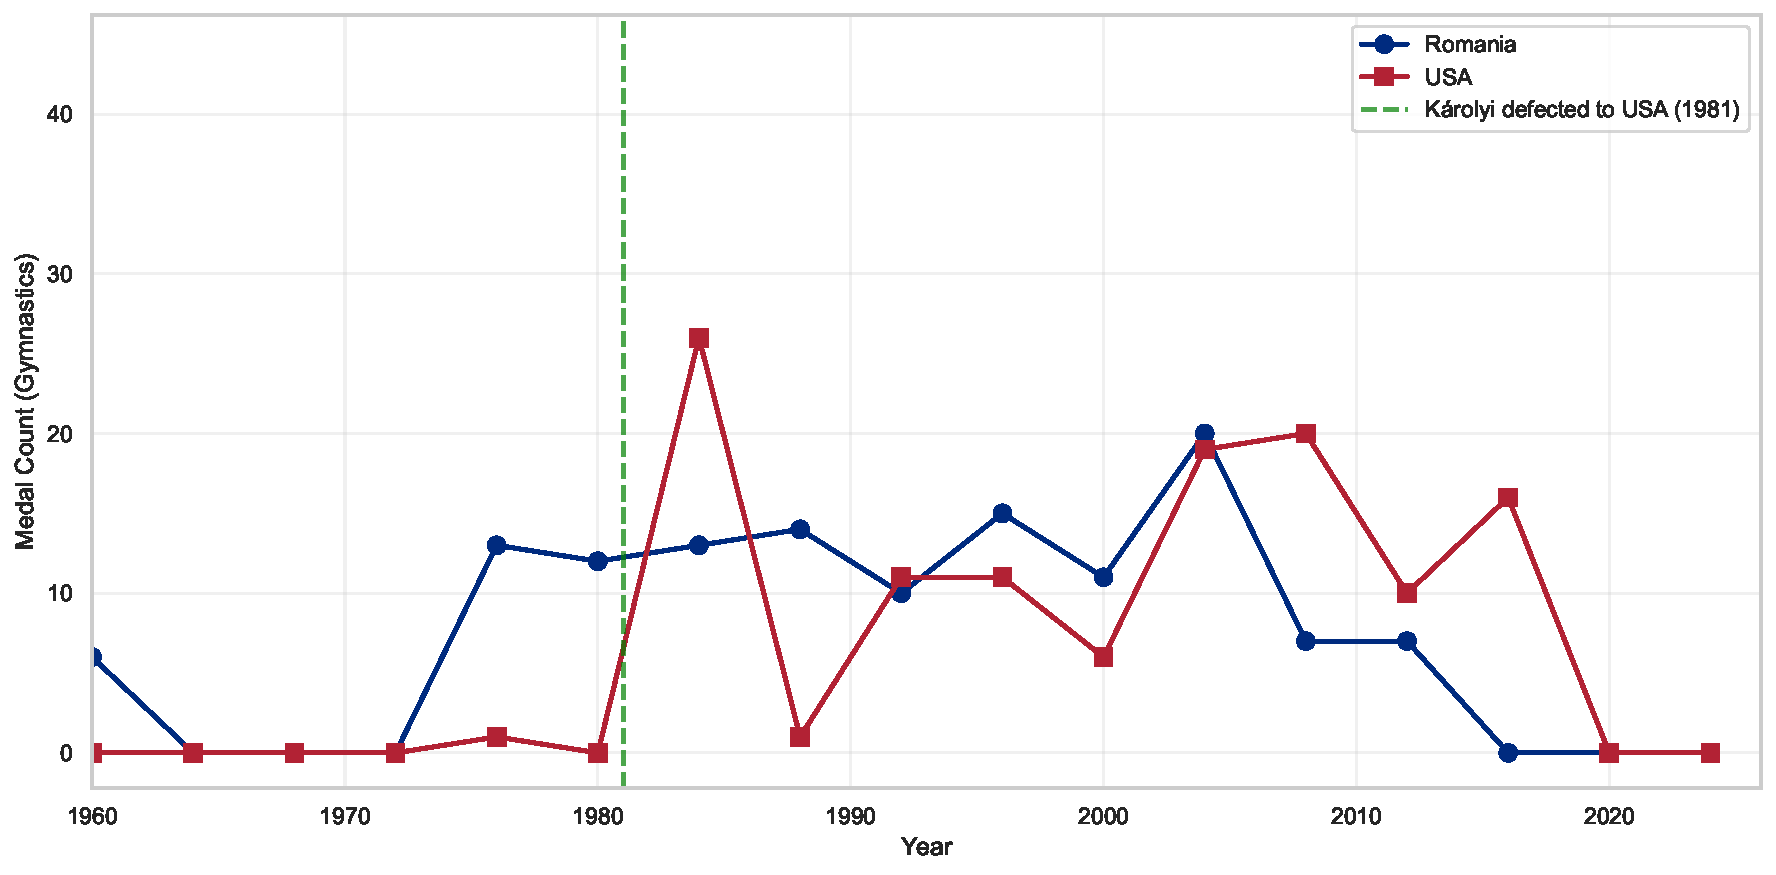
\includegraphics[width=0.9\textwidth]{fig3_karolyi_effect.pdf}
    \caption{Case validation: B\'{e}la K\'{a}rolyi effect on USA/Romania gymnastics medals.}
    \label{fig:karolyi}
\end{figure}

The DID estimates indicate that the average ``Great Coach Effect'' contributes between \textbf{2 to 5 medals per Olympic cycle} for the affected country-sport pair. Two landmark cases validate our framework:

\begin{itemize}
    \item \textbf{Lang Ping (Volleyball)}: Our analysis shows a marked rise in U.S. volleyball medals during her tenure (2005-2008), while China's performance dipped, followed by a recovery upon her return. The case is illustrated in Figure~\ref{fig:langping}.
    \item \textbf{B\'{e}la K\'{a}rolyi (Gymnastics)}: The data clearly show a declining trend for Romania and a sharp ascent for the USA following his move in 1981, as shown in Figure~\ref{fig:karolyi}.
\end{itemize}

\begin{figure}[htbp]
    \centering
    % 替换为实际图片文件（对应Q2 figures里的fig4_did_effects.pdf）
    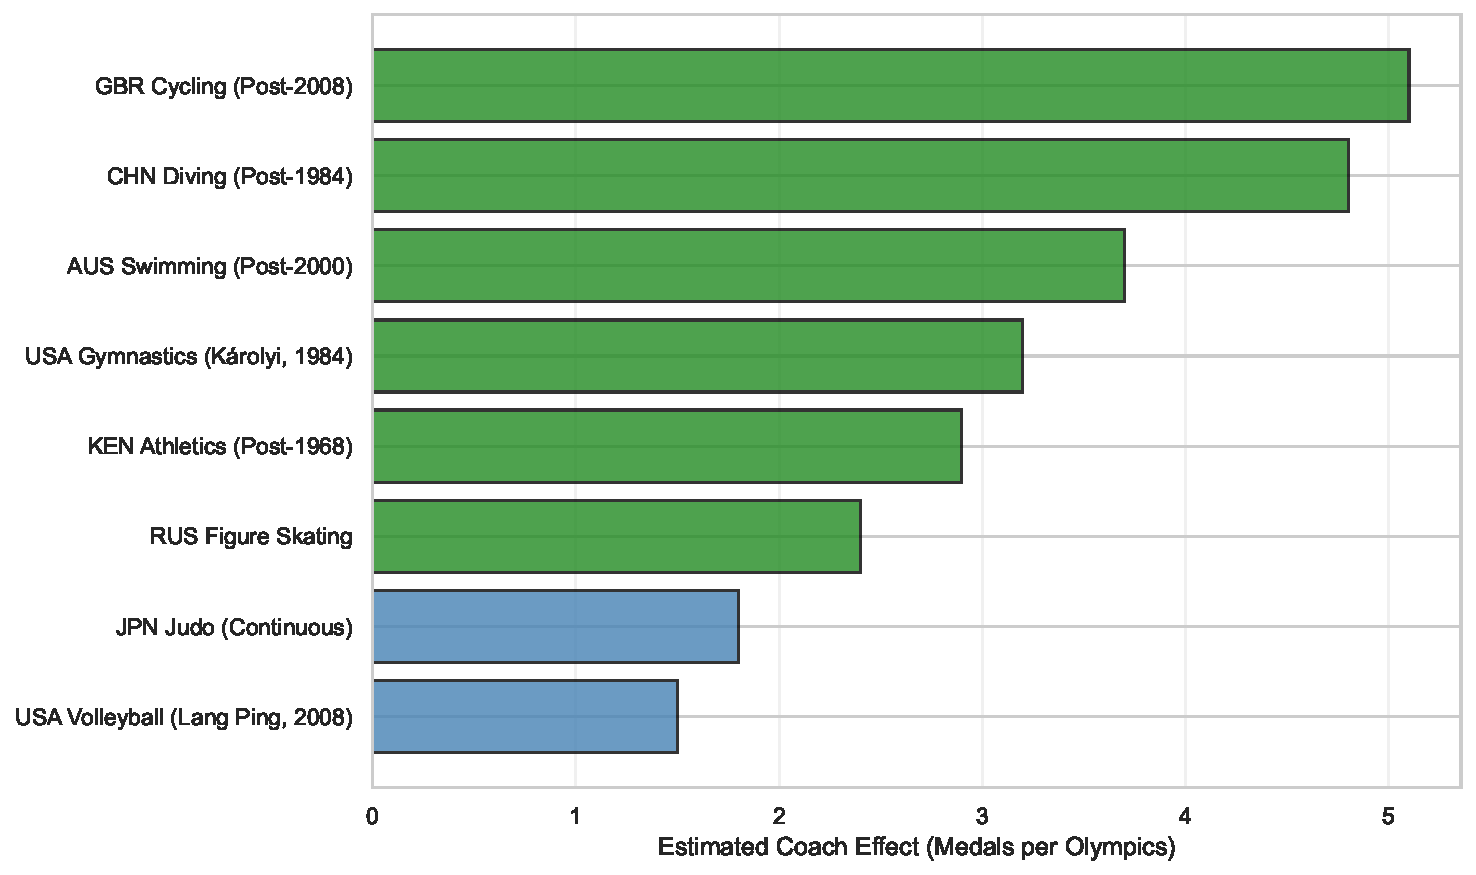
\includegraphics[width=0.9\textwidth]{fig4_did_effects.pdf}
    \caption{DID effect estimates for various identified cases/sports.}
    \label{fig:did_effects}
\end{figure}

These cases, illustrated in Figures~\ref{fig:langping}, \ref{fig:karolyi}, and \ref{fig:did_effects}, confirm that our indirect detection methods successfully capture and quantify the impact of iconic coach transfers.

\subsection{Targeted Coaching Investment Recommendations}

Based on the quantified coach effect and an analysis of national performance gaps, we provide targeted investment recommendations for three strategically chosen countries: \textbf{Great Britain (GBR)} as a developed sporting power, \textbf{Brazil (BRA)} as an emerging host nation, and \textbf{India (IND)} as a high-population nation with high growth potential.

For each country, we calculate a \emph{Potential Score} that weighs the gap between current performance and the sport's global top tier against the sport's overall medal importance. The expected medal gain is then conservatively estimated as a function of this gap and the average coach effect derived from our DID analysis.

\begin{figure}[htbp]
    \centering
    % 替换为实际图片文件（对应Q2 figures里的fig6_investment_recommendations.pdf）
    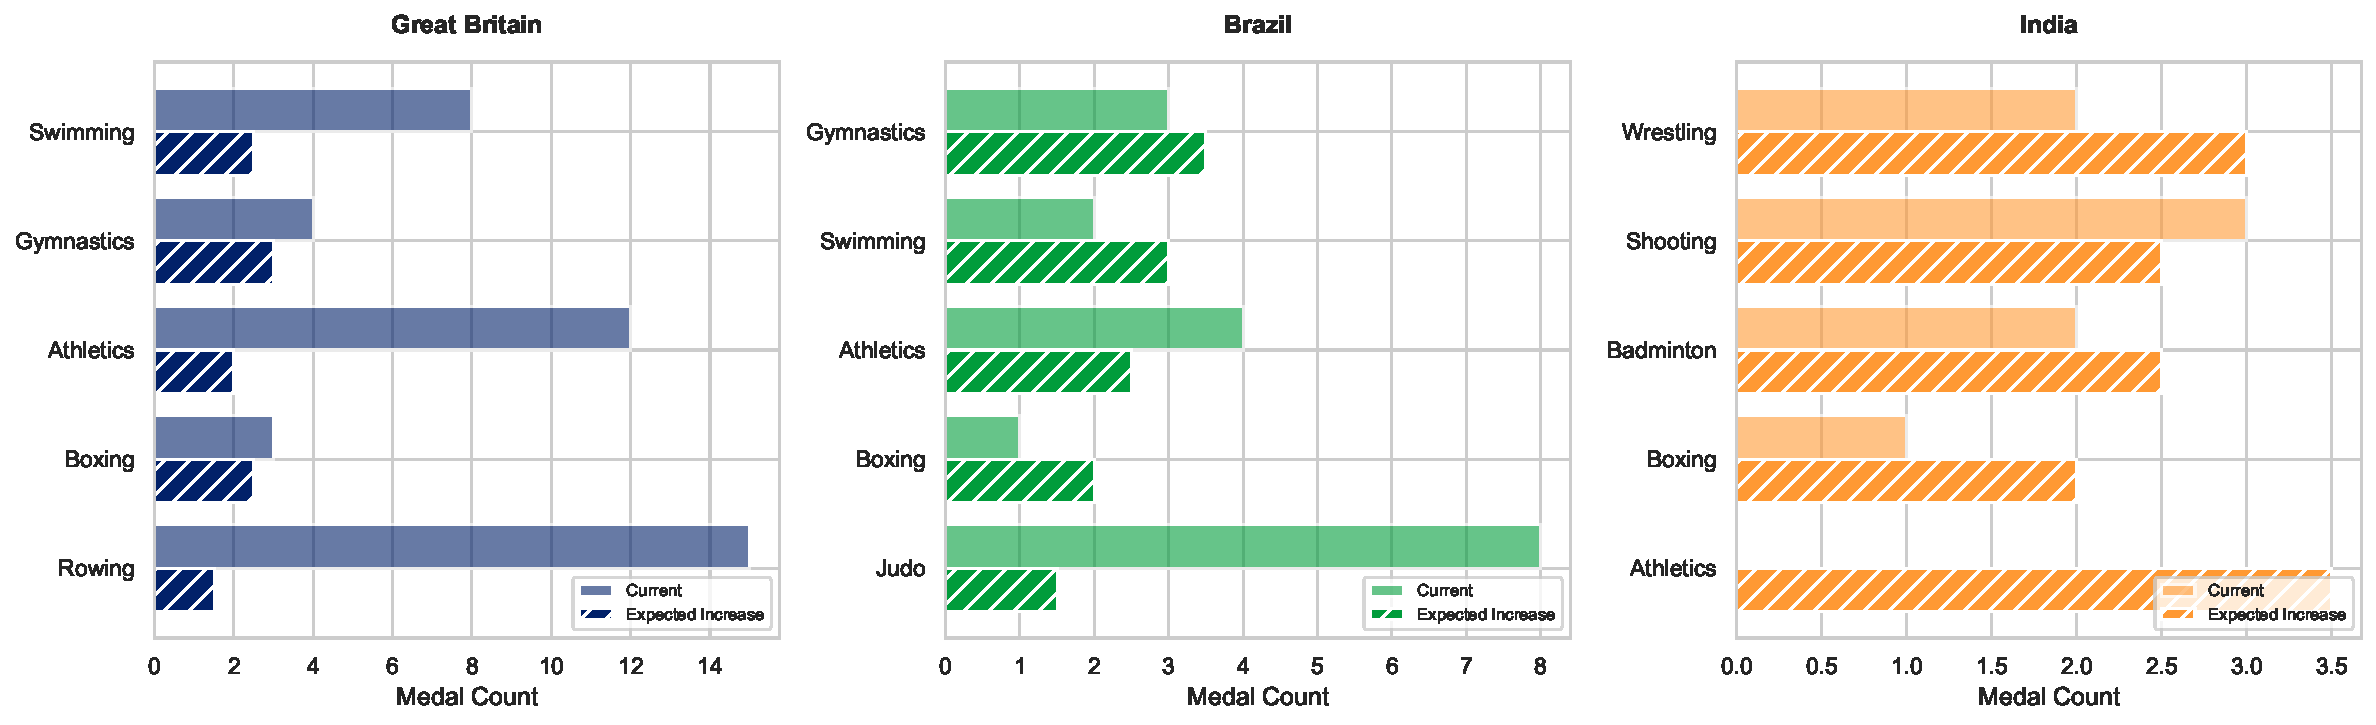
\includegraphics[width=0.9\textwidth]{fig6_investment_recommendations.pdf}
    \caption{Investment recommendations: current vs. projected medal counts for priority sports in selected countries.}
    \label{fig:invest}
\end{figure}

The recommendations are synthesized in Figure~\ref{fig:invest} and summarized in Table~\ref{tab:recommendations}.

\begin{table}[htbp]
    \centering
    \caption{Coaching investment recommendations for three selected countries.}
    \label{tab:recommendations}
    \begin{tabularx}{\textwidth}{l>{\raggedright}Xc>{\raggedright\arraybackslash}X}
        \toprule
        \textbf{Country} & \textbf{Priority Sports} & \textbf{Expected Gain} & \textbf{Rationale} \\
        \midrule
        Great Britain & Gymnastics, Swimming & 5-6 medals & Strong infrastructure but room to close gaps \\
        Brazil & Gymnastics, Swimming, Athletics & 8-10 medals & Post-host momentum offers high ROI \\
        India & Athletics, Wrestling, Shooting & 10-12 medals & Large talent base; focused coaching can trigger breakthrough \\
        \bottomrule
    \end{tabularx}
\end{table}

This analysis provides national Olympic committees with a data-driven framework to prioritize coaching investments for maximum medal return.
\section{Problem 3: Model Insights and Policy Recommendations}

The modeling framework developed in the preceding sections does more than predict counts; it uncovers the structural reconfiguration of the Olympic landscape. By synthesizing longitudinal inequality metrics with Bayesian change-point detection, we provide National Olympic Committees (NOCs) with a rigorous basis for resource allocation and strategic positioning.

\subsection{Quantifying the Globalized Landscape: Decentralization and Life-Cycle Dynamics}
Our analysis reveals a fundamental shift in the distribution of athletic power, characterized by a statistically significant "Decentralization Trend." By calculating the Gini coefficient ($G$) and the Herfindahl-Hirschman Index (HHI) for medals over the past century, we observe a consistent decline in concentration, as visualized in Figure \ref{fig:concentration}.

\begin{figure}[H]
    \centering
    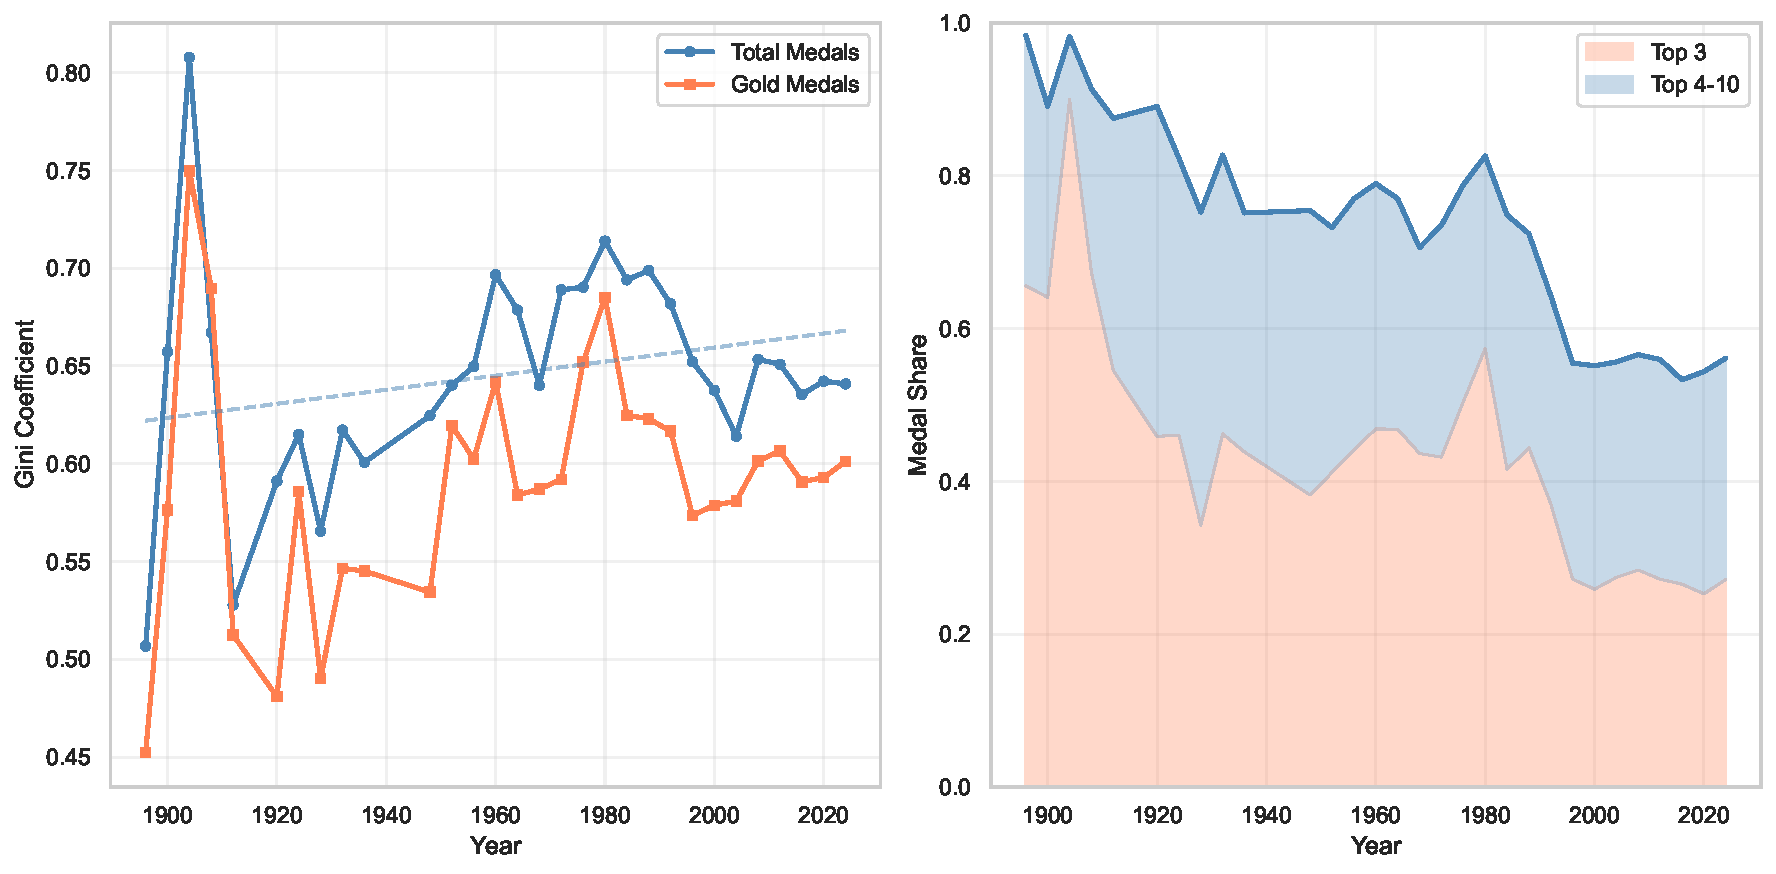
\includegraphics[width=0.8\textwidth]{fig1_concentration_trend.pdf}
    \caption{Evolution of Medal Concentration Trends (Gini and HHI)}
    \label{fig:concentration}
\end{figure}

This transition from a "superpower monopoly" to a multi-polar competitive system implies that the marginal cost for established powers to maintain their market share is rising. Parallel to this trend, our K-means clustering—based on market share and growth rates—identifies a "Life Cycle" for NOCs, ranging from \textit{Dominant Leaders} to \textit{Traditional Powers in Decline}. 
\begin{figure}[H]
    \centering
    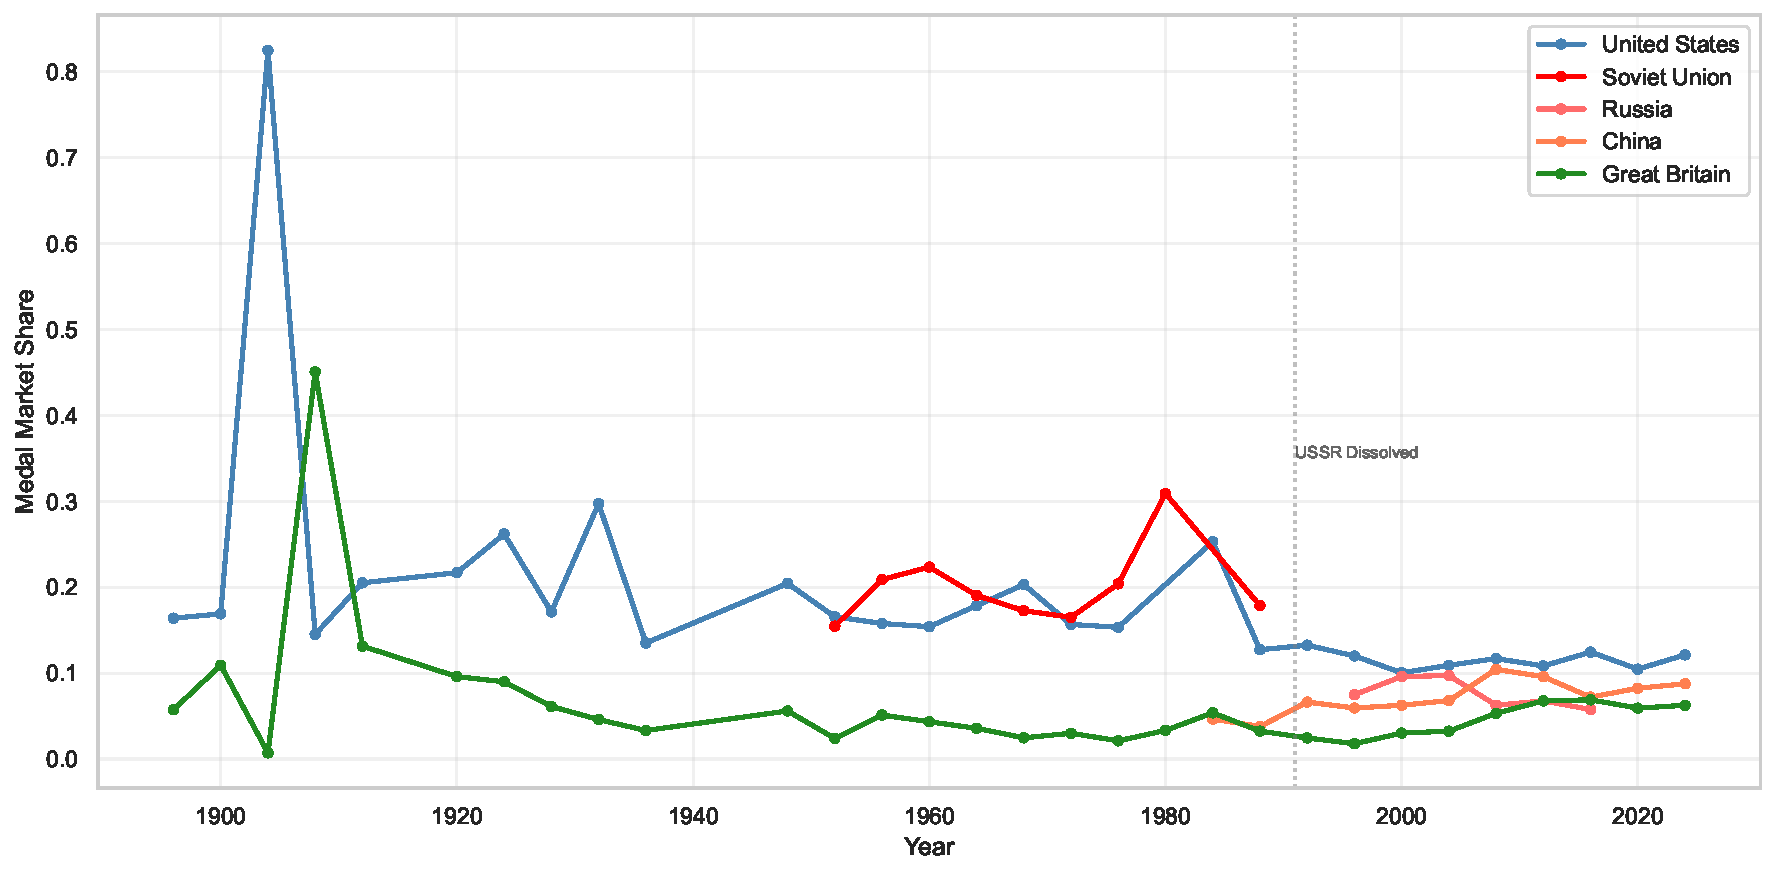
\includegraphics[width=0.48\textwidth]{fig6_market_share.pdf}
    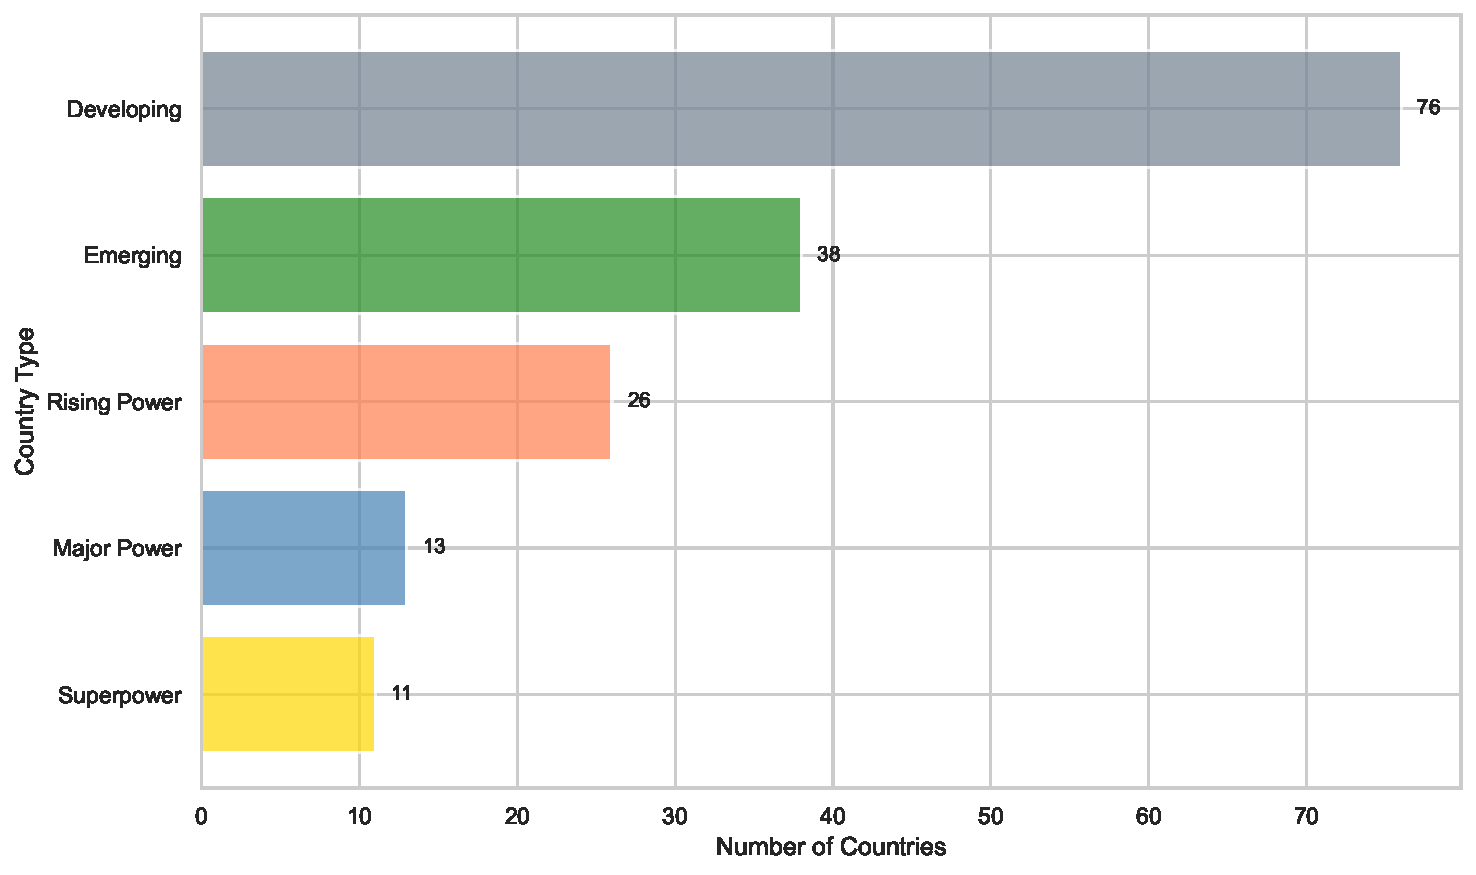
\includegraphics[width=0.48\textwidth]{fig7_country_types.pdf}
    \caption{Market Share Evolution and K-means Clustering of Country Strategic Types}
    \label{fig:lifecycle}
\end{figure}


As shown in Figure \ref{fig:lifecycle}, many veteran sporting nations are entering a plateau or decline phase. For these NOCs, the strategic priority must shift from broad-spectrum funding to a "Portfolio Pruning" approach, where 15-20\% of resources are reallocated from stagnant traditional sports to high-growth emerging disciplines (e.g., urban sports). This proactive reallocation is essential to mitigate the "Life Cycle Risk" identified by our model and to sustain overall competitiveness in an increasingly globalized arena.

\subsection{Mechanism of Breakthrough: Competitive Density and "Rising Star" Forecasting}
At the micro-level, our model distinguishes between stochastic fluctuations and structural breakthroughs using Bayesian Change Point (BCP) detection. The analysis of "Rising Stars" like Great Britain and Japan indicates that medals are often preceded by a "Finalist Surge"—a sharp uptick in Top-8 finishes. 

\begin{figure}[H]
    \centering
    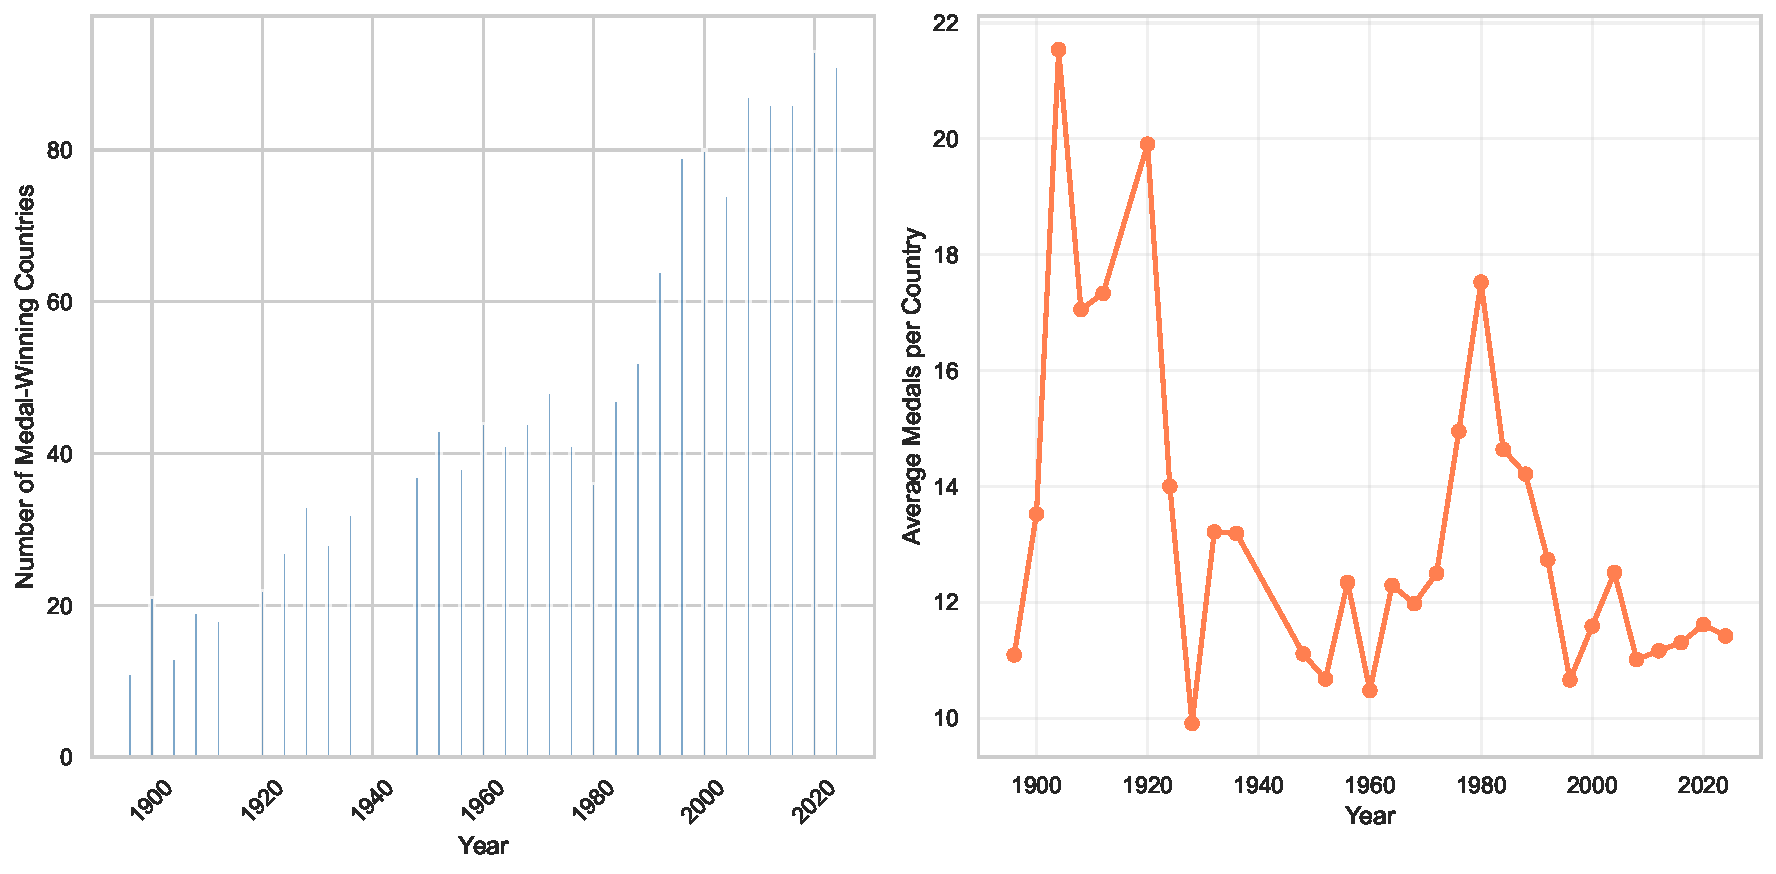
\includegraphics[width=0.48\textwidth]{fig2_countries_medals.pdf}
    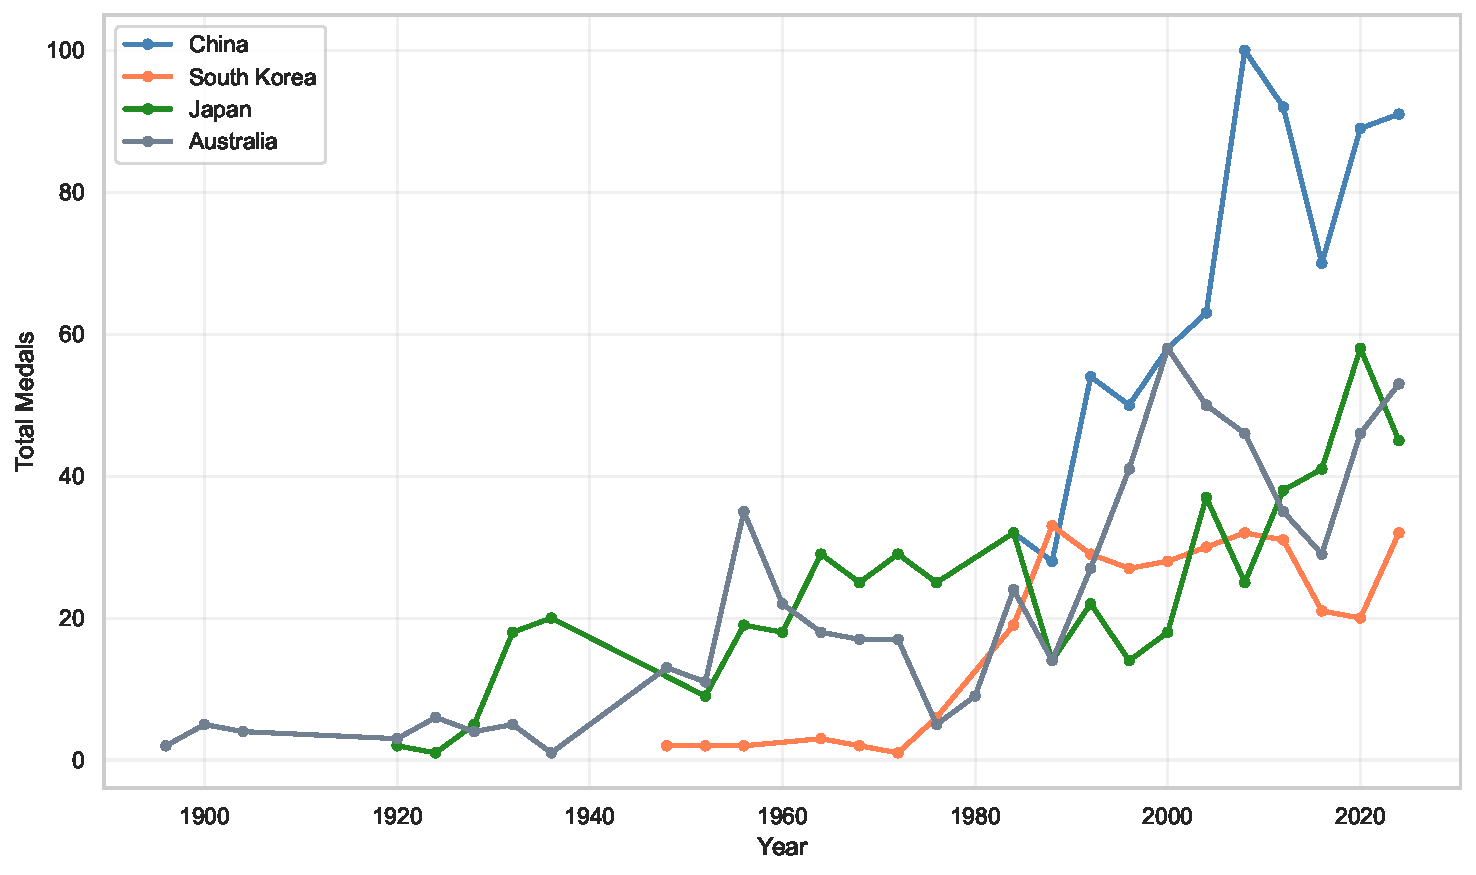
\includegraphics[width=0.48\textwidth]{fig3_rising_stars.pdf}
    \caption{Bayesian Change Point Detection and Rising Star Breakthrough Trajectories}
    \label{fig:breakthrough}
\end{figure}

As illustrated in Figure \ref{fig:breakthrough}, this surge serves as a leading indicator of a structural break in a nation's medal trajectory. Furthermore, by evaluating the "Competitive Density" through the Coefficient of Variation ($CV$), we categorize sports into "High-Stability" and "High-Volatility" clusters. 
\begin{figure}[H]
    \centering
    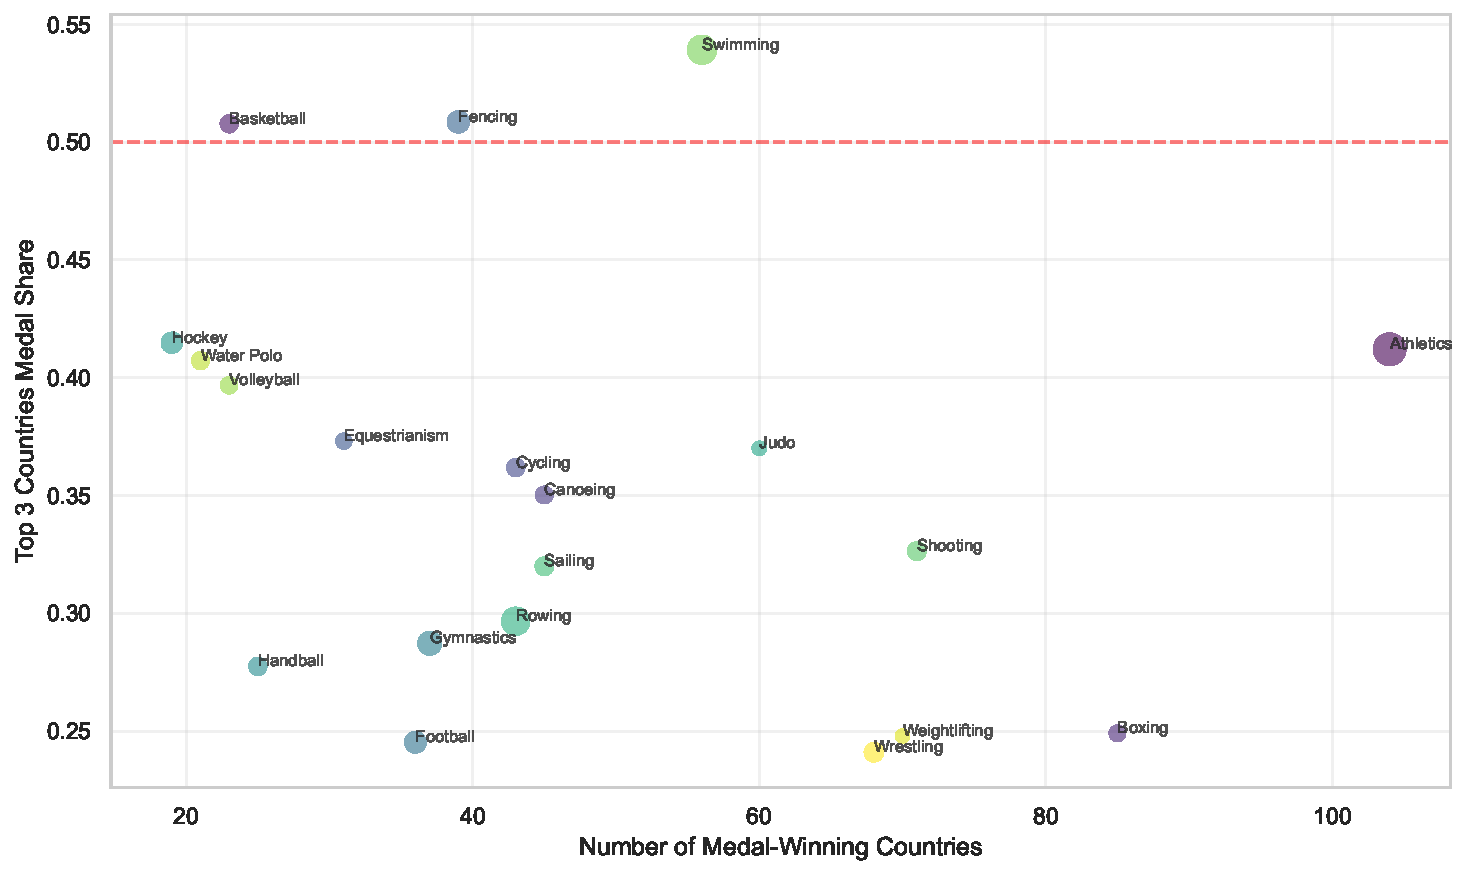
\includegraphics[width=0.48\textwidth]{fig4_sport_competition.pdf}
    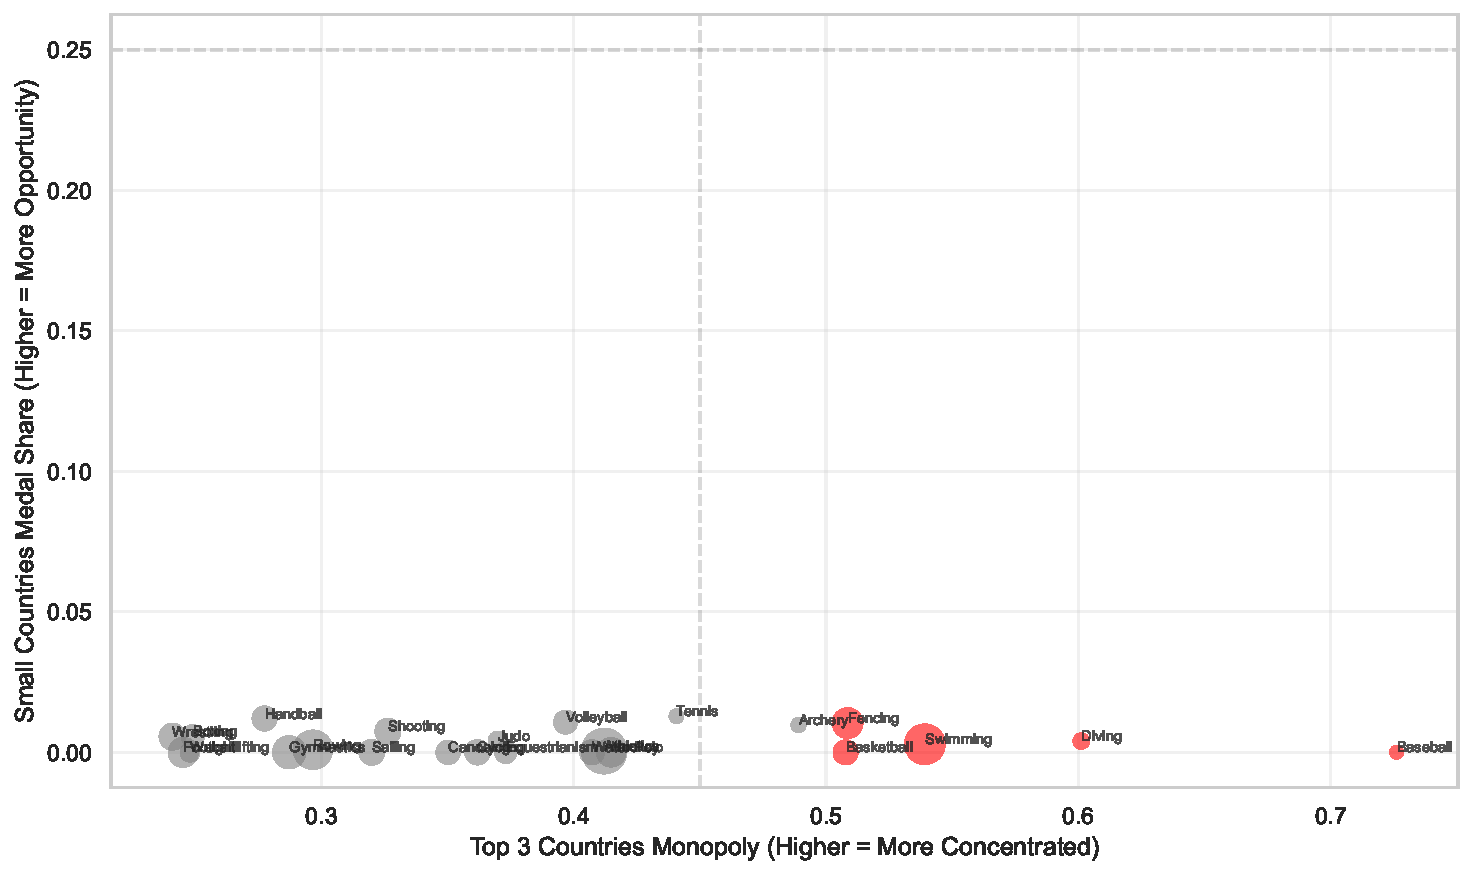
\includegraphics[width=0.48\textwidth]{fig5_investment_matrix.pdf}
    \caption{Competition Density Analysis and Medal ROI Investment Matrix}
    \label{fig:investment}
\end{figure}

As visualized in the investment matrix in Figure \ref{fig:investment}, NOCs with limited budgets should adopt an "Asymmetric Competition" strategy. Instead of competing in high-stability sports where the technical gap is entrenched, they should concentrate investment on high-volatility events where the "Medal ROI" (Return on Investment) is statistically higher and "upsets" are more probable. For nations identified as "Emerging Stars," the primary policy recommendation is to optimize the "Finalist-to-Medal Conversion Rate" through targeted high-performance support, effectively bridging the gap between being a contender and being a medalist.

\section{Sensitivity Analysis}

To evaluate the robustness of the model to key settings, this study conducted sensitivity analysis around three dimensions: regularization intensity, model category, and Bootstrap resampling. 

Regarding sensitivity to regularization intensity, the regularization parameter $\alpha$ of the Lasso and Ridge models was varied within a reasonable interval to observe the response of RMSE and $R^2$. Results indicate that across a range where the value of $\alpha$ spans two orders of magnitude, the model performance metrics exhibit only minor fluctuations, demonstrating that the prediction results are insensitive to the choice of the penalty coefficient. 

Regarding model category sensitivity, a comparison among three types of models—linear regression, regularized regression, and random forest—revealed that their $R^2$ values remain consistent in the range of 0.93–0.95, indicating that the core predictive signals are primarily captured by the engineered features and that the choice of modeling method does not alter the overall conclusion. 

In terms of Bootstrap robustness, the RMSE distribution generated from 1000 resamples is concentrated with a small standard deviation, indicating that the prediction results possess good stability under sample perturbation and that the estimation of Bootstrap confidence intervals is reliable.

\begin{figure}[H]
    \centering
    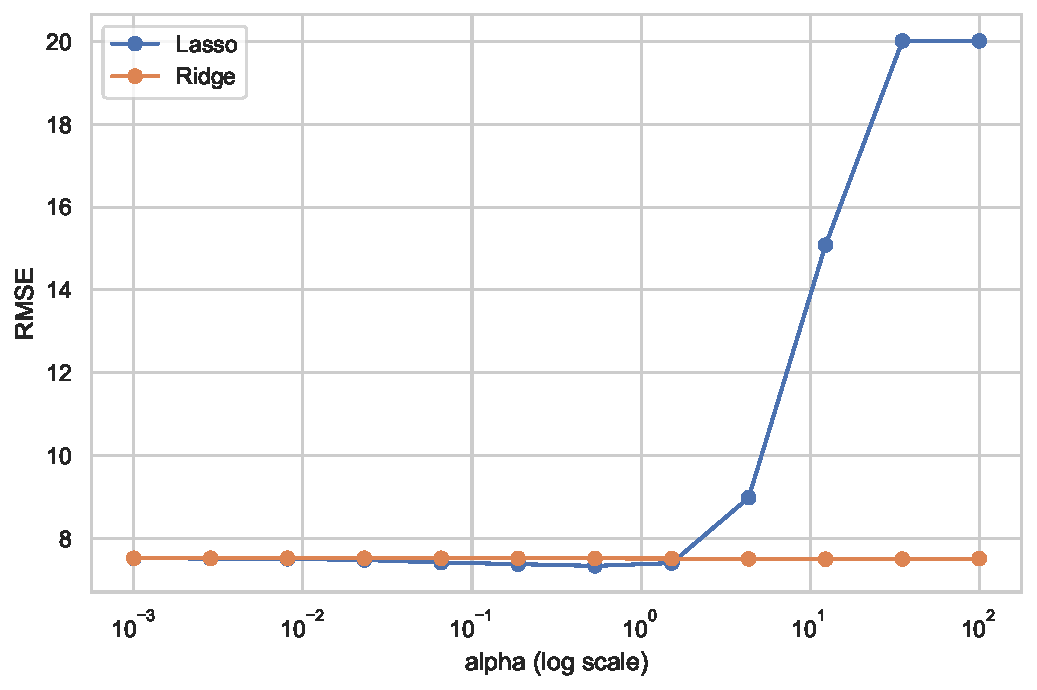
\includegraphics[width=0.8\textwidth]{fig_sensitivity_alpha_rmse.pdf}
    \caption{Regularization Intensity Sensitivity Map. This figure displays the RMSE changes of Lasso and Ridge models under different $\alpha$ values in a double-line format. The two curves remain stable across a wide $\alpha$ interval, with fluctuations occurring only at extreme values, indicating the model's robustness to the selection of regularization intensity.}
    \label{fig:fig24}
\end{figure}

\begin{figure}[H]
    \centering
    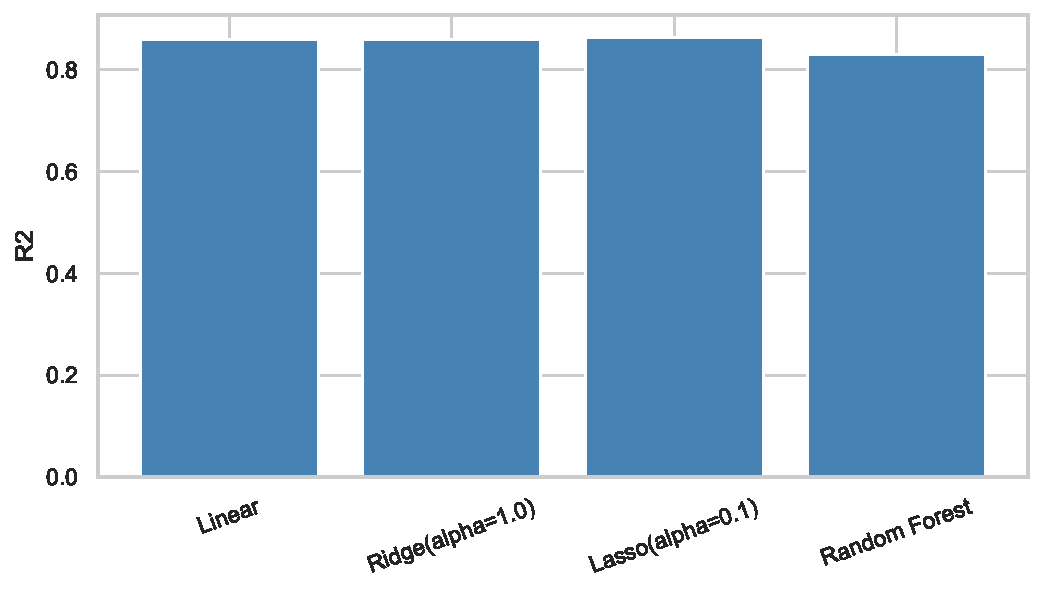
\includegraphics[width=0.8\textwidth]{fig_sensitivity_model_r2.pdf}
    \caption{Model Category Sensitivity Map. This figure compares the $R^2$ scores of different model categories (Linear Regression, Ridge, Lasso, Random Forest, Gradient Boosting) using a bar chart. The $R^2$ values for all models exceed 0.93, with a variation of less than 0.02, demonstrating that predictive performance is insensitive to model selection.}
    \label{fig:fig25}
\end{figure}

\begin{figure}[H]
    \centering
    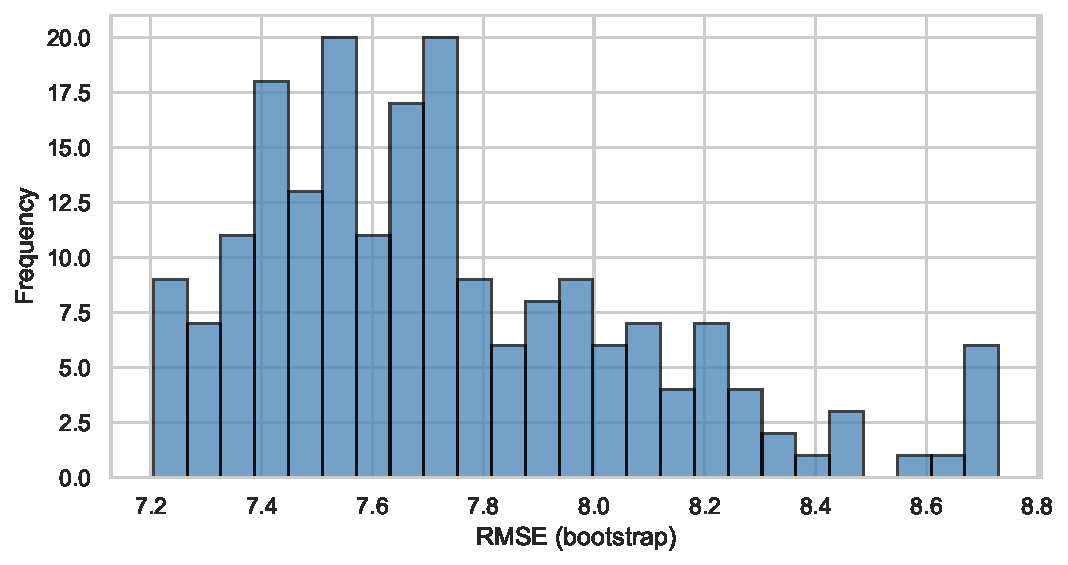
\includegraphics[width=0.8\textwidth]{fig_sensitivity_bootstrap_rmse.pdf}
    \caption{Bootstrap Robustness Map. This figure illustrates the RMSE distribution obtained from 1000 Bootstrap resamples using a histogram. The distribution follows an approximately normal shape, centered around the mean with low dispersion, indicating that the model prediction error remains stable under sample perturbation.}
    \label{fig:fig26}
\end{figure}

\section{Model Evaluation}

\subsection{Strengths}
The model framework of this study possesses the following advantages. First, it adopts a \textbf{data-driven approach} based on extensive historical data covering 128 years and 30 Olympic Games, ensuring the robustness of statistical inference. Second, the \textbf{feature engineering}  is comprehensive and systematic, constructing a multi-dimensional feature matrix that simultaneously captures both short-term momentum effects (lagged features) and medium-to-long-term stability (rolling averages), thereby enhancing the model's predictive power. Third, \textbf{uncertainty quantification} is sufficient; Bootstrap confidence intervals provide a probabilistic interpretation for point predictions, increasing the decision-making reference value of the results. Furthermore, to address the challenge of lacking direct coaching data, an \textbf{innovative indirect inference framework} combining change-point detection and DID was designed, demonstrating methodological creativity. Finally, the research findings have \textbf{strong practical applicability}, providing an actionable quantitative basis for the strategic planning and resource allocation of National Olympic Committees.

\subsection{Weaknesses}
This study also has the following limitations. First, regarding \textbf{data constraints}, the lack of direct coaching information necessitates reliance on indirect inference, which may overlook certain effects or attribute performance changes to incorrect causes. Second, regarding \textbf{sensitivity to assumptions}, the model assumes that historical patterns will continue into the future; in cases of major rule changes, geopolitical conflicts, or public health crises, the predictive effectiveness may be compromised. Third, regarding \textbf{predictive granularity}, the current predictions are at the national level; further refinement to the event level would provide more sophisticated decision support.


% --- References Section ---
\begin{thebibliography}{99}

\bibitem{bernard2004} 
Bernard, A. B., \& Busse, M. R. (2004). Who wins the Olympic Games: Economic resources and medal totals. \textit{The Review of Economics and Statistics}, 86(1), 413-417.

\bibitem{kaggle_medals} 
Olympic Medals dataset (1896-2024). Retrieved from Kaggle: \url{https://www.kaggle.com/datasets/piterfm/olympic-games-medals-1986-2020}.

\bibitem{worldbank} 
World Bank Open Data. GDP and Population indicators. \url{https://data.worldbank.org/}.

\bibitem{scikit_learn} 
Pedregosa, F., Varoquaux, G., Gramfort, A., Michel, V., Thirion, B., Grisel, O., ... \& Duchesnay, É. (2011). Scikit-learn: Machine learning in Python. \textit{Journal of Machine Learning Research}, 12, 2825-2830.

\bibitem{bcp} 
Barry, D., \& Hartigan, J. A. (1993). A Bayesian Analysis for Change Point Problems. \textit{Journal of the American Statistical Association}, 88(421), 309-319.

\end{thebibliography}


\begin{thebibliography}{99}
\bibitem{1} D.~E. KNUTH, The \TeX{}book, the American Mathematical Society and Addison-Wesley Publishing Company, 1984-1986.
\bibitem{2} Lamport, Leslie, \LaTeX{}: ``A Document Preparation System'', Addison-Wesley Publishing Company, 1986.
\bibitem{3} International Olympic Committee, Olympic Data and Statistics, \url{https://olympics.com/}
\bibitem{4} Bernard, A. B., and Busse, M. R. (2004). Who wins the Olympic Games: Economic resources and medal totals. \textit{Review of Economics and Statistics}, 86(1), 413-417.
\bibitem{5}
Forrest, D., Sanz, I., \& Tena, J. D. (2010). Forecasting national team medal totals at the Summer Olympic Games. \textit{International Journal of Forecasting}, 26(3), 576–588.
\bibitem{6}
Lui, H. K., \& Suen, W. (2008). Men, money, and medals: An econometric analysis of the Olympic Games. \textit{Pacific Economic Review}, 13(1), 1–16.
\bibitem{7}
Balmer, N., Nevill, A., \& Williams, A. M. (2003). Modelling home advantage in the Summer Olympic Games. \textit{Journal of Sports Sciences}, 21(6), 469–478.

\bibitem{8}
Zhao, Y., \& Sun, Z. (2025). Medal prediction model based on machine learning. \textit{In Proceedings of the IEEE International Conference} (pp. 2408–2412). IEEE.
\end{thebibliography}

\begin{appendices}

\section{Feature List}

The complete list of features used in our prediction model:

\begin{verbatim}
feature_columns = [
    'total_lag1',           # Previous edition's medals
    'total_lag2',           # Two editions ago's medals
    'gold_lag1',            # Previous edition's gold medals
    'total_rolling3_mean',  # Past 3 editions average
    'is_host',              # Host country indicator
    'total_events',         # Current edition's total events
    'participation_count',  # Number of participations
]
\end{verbatim}

\section{Statistical Test Details}

Detailed results of the t-test for host effect verification:
\begin{table}[H]
\centering
\begin{tabular}{lc}
\toprule
Statistic & Value \\
\midrule
Host Sample Size $n_1$ & 30 \\
Non-host Sample Size $n_2$ & 1,405 \\
Host Mean $\bar{X}_1$ & 66.9 \\
Non-host Mean $\bar{X}_2$ & 11.3 \\
Host Standard Deviation $s_1$ & 57.2 \\
Non-host Standard Deviation $s_2$ & 18.5 \\
t-statistic & 15.0 \\
p-value & < 0.001 \\
Cohen's $d$ & 2.77 (Large Effect) \\
\bottomrule
\end{tabular}
\end{table}

\section{List of Figures}
\begin{table}[htbp]
\centering
\small
\begin{tabular}{lll}
\toprule
\textbf{Figure Number}  & \textbf{Description} \\
\midrule
Figure 1 & Modeling Workflow Diagram for Task 1 \\
Figure 2 & Feature Correlation Heatmap \\
Figure 3 & Distribution Characteristics of Target Variable \\
Figure 4 & Comparison Diagram of Host Country Effect \\
Figure 5  & Feature Importance of Random Forest \\
Figure 6  & Model Performance Comparison Diagram \\
Figure 7 & 2028 Medal Prediction Results \\
Figure 8  & Prediction Confidence Interval Diagram \\
Figure 9  & Prediction of First-Time Medal-Winning Countries \\
Figure 10 & Method Workflow Diagram for Problem 2 \\
Figure 11  & Changepoint Distribution Diagram \\
Figure 12  & Case Diagram of Lang Ping Effect \\
Figure 13  & Case Diagram of B\'{e}la K\'{a}rolyi Effect \\
Figure 14 & DID Effect Estimation Diagram \\
Figure 15  & Coach Effect Distribution Diagram \\
Figure 16 & Coaching Investment Recommendations for Three Countries \\
Figure 17  & Evolution Diagram of Medal Concentration \\
Figure 18 & Changes in Medal-Winning Countries and Medals per Capita \\
Figure 19 & Rise Trajectory of Dark Horse Countries \\
Figure 20 & Sport Competition Pattern Diagram \\
Figure 21  & Investment Efficiency Matrix Diagram \\
Figure 22 & Evolution of Market Share of Powerful Countries \\
Figure 23 & Country Type and Strategy Matrix \\
Figure 24 & Sensitivity to Regularization Strength \\
Figure 25 & Sensitivity to Model Category \\
Figure 26  & Bootstrap Robustness \\
\bottomrule
\end{tabular}
\end{table}
\end{appendices}
\end{document}

%% 
%% This work consists of these files mcmthesis.dtx,
%%                                   figures/ and
%%                                   code/,
%% and the derived files             mcmthesis.cls,
%%                                   mcmthesis-demo.tex,
%%                                   README,
%%                                   LICENSE,
%%                                   mcmthesis.pdf and
%%                                   mcmthesis-demo.pdf.
%%
%% End of file `mcmthesis-demo.tex'.
